% =====================================================================
% Experimental sections for the LCN credal-inference paper.
%
% This file SUPERSEDES the \section{Experiments} currently in
% docs/paper/neurips_2026.tex (around line 564), which describes an earlier
% experiment generation (CCTE / CCTE_cm, hand-pasted numbers, figs/small-dag_*
% figures, Exact/ARIEL references). Everything here is derived from the current
% results in outputs/ and plots/, with CredalJT as the uniform reference.
%
% BUILD (from the repository root, so that plots/ and outputs/ resolve):
%     TEXINPUTS=docs/paper: pdflatex -interaction=nonstopmode docs/experiments.tex
%     TEXINPUTS=docs/paper: bibtex   experiments        (if citations are needed)
%     TEXINPUTS=docs/paper: pdflatex -interaction=nonstopmode docs/experiments.tex
%
% Section 1 is the main-paper section and is held to 2 pages in this layout.
% Section 2 is the appendix section and has no page limit.
% =====================================================================
\documentclass{article}

\usepackage{neurips_2026}          % found via TEXINPUTS=docs/paper:
\usepackage[utf8]{inputenc}
\usepackage[T1]{fontenc}
\usepackage{hyperref}
\usepackage{url}
\usepackage{booktabs}
\usepackage{amsfonts}
\usepackage{microtype}
\usepackage{graphicx}
\usepackage{subcaption}
\usepackage{amsmath}
\usepackage{amssymb}
\usepackage{times}
\usepackage{multirow}

\graphicspath{{plots/}{../plots/}{docs/paper/figs/}}

% No \maketitle: these sections are meant to be dropped into the paper body, so
% the page budget below measures the section content only.
\pagestyle{plain}

% Allow the two floats of Section 1 to share a page with text rather than
% spilling onto a third page.
\renewcommand{\topfraction}{0.9}
\renewcommand{\bottomfraction}{0.6}
\renewcommand{\textfraction}{0.07}
\renewcommand{\floatpagefraction}{0.85}
\setcounter{topnumber}{2}
\setcounter{bottomnumber}{2}
\setcounter{totalnumber}{4}

\begin{document}

%% ================================================================
\section{Experiments}
\label{sec-experiments}
%% ================================================================

\begin{figure}[!t]
    \centering
    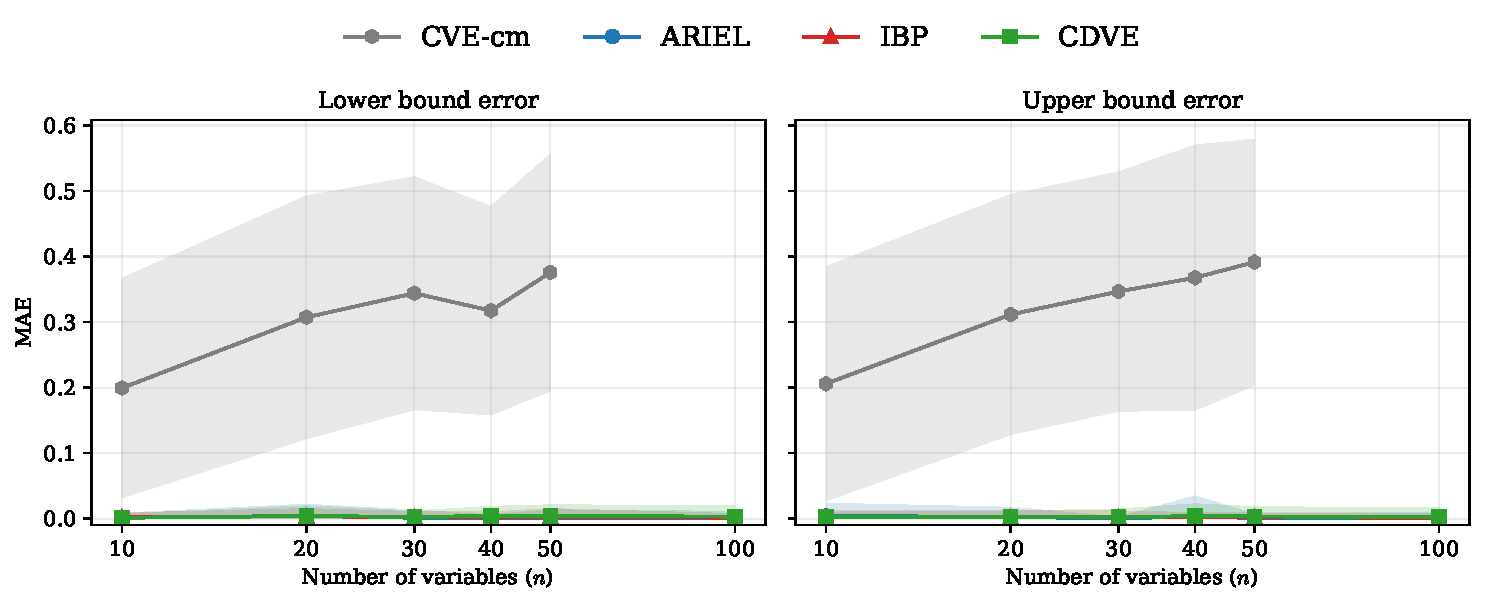
\includegraphics[width=0.80\linewidth]{dag_large_fr_mae.pdf}
    \caption{Large random \texttt{dag} LCNs (loopy, treewidth $\le 3$): MAE against
    the CredalJT reference, with bands giving one standard deviation over the ten
    instances per size and curves stopping where the budget was exceeded. Timings
    and the other three families are in Appendix~\ref{sec-full-results}.}
    \label{fig:random}
\end{figure}

\begin{table}[!b]
\centering
\footnotesize
\begin{tabular}{llrrrr}
\toprule
Instance & Algorithm & MAE$_{l}$ & MAE$_{u}$ & $w$ & Time (s) \\
\midrule
Alarm ($n{=}10$), ref 0.72s & ARIEL & 0.000 & 0.000 & 1.00 & 3.92 \\
 & IBP & 0.101 & 0.015 & 1.37 & 0.13 \\
 & CDVE & 0.101 & 0.015 & 1.37 & 0.69 \\
 & CVE$_{cm}$ & 0.087 & 0.067 & 0.86 & 0.24 \\
\hline
Credit ($n{=}11$), ref 1.15s & ARIEL & 0.050 & 0.000 & 1.18 & 3.18 \\
 & IBP & 0.257 & 0.000 & 1.92 & 0.24 \\
 & CDVE & 0.257 & 0.000 & 1.92 & 0.69 \\
 & CVE$_{cm}$ & 0.108 & 0.165 & 0.78 & 1.73 \\
\hline
Hepatitis ($n{=}10$), ref 0.56s & ARIEL & 0.008 & 0.008 & 1.02 & 3.91 \\
 & IBP & 0.069 & 0.080 & 1.86 & 0.75 \\
 & CDVE & 0.070 & 0.085 & 1.85 & 1.15 \\
 & CVE$_{cm}$ & 0.114 & 0.184 & 1.49 & 16.53 \\
\hline
MScaling ($n{=}12$), ref 0.66s & ARIEL & 0.028 & 0.000 & 1.73 & 8.13 \\
 & IBP & 0.129 & 0.493 & 7.64 & 0.35 \\
 & CDVE & 0.129 & 0.501 & 7.72 & 1.23 \\
 & CVE$_{cm}$ & 0.079 & 0.227 & 2.99 & 0.57 \\
\hline
BScaling ($n{=}32$), ref 2.42s & ARIEL & 0.000 & 0.000 & 1.00 & 19.80 \\
 & IBP & 0.115 & 0.225 & 4.49 & 0.69 \\
 & CDVE & 0.115 & 0.225 & 4.49 & 20.55 \\
 & CVE$_{cm}$ & 0.064 & 0.072 & 1.55 & 9.18 \\
\hline
PScaling ($n{=}40$), ref 3.27s & ARIEL & 0.000 & 0.000 & 1.00 & 34.72 \\
 & IBP & 0.129 & 0.263 & 4.43 & 0.91 \\
 & CDVE & 0.129 & 0.263 & 4.43 & 51.25 \\
 & CVE$_{cm}$ & 0.070 & 0.057 & 1.20 & 658.84 \\
\bottomrule
\end{tabular}
\caption{Realistic LCNs: three instances derived from real Bayesian networks
(top) and three Supreme Court chain-graph instances (bottom), all against the
CredalJT reference. $w$ is the mean interval-width ratio ($>1$ looser than the
reference, $<1$ tighter). Time is total time including the
credal-network build; the reference's own time on each instance is given with the
instance name.}
\label{tab:real}
\end{table}

\paragraph{Benchmarks.}
We evaluate on two groups of instances. \emph{Random LCNs} come in four
families, each generated so that every sentence is \emph{family-realizable}:
\texttt{tree}, \texttt{polytree}, \texttt{ktree} ($k{=}3$) and \texttt{dag}
(moralized treewidth $\le 3$, at most two parents per atom). Family-realizability means each sentence constrains a single family's conditional
table alone; with the \texttt{linear} factorization the credal-network relaxation
is exact \emph{iff} the primal graph is singly connected \emph{and} every sentence
is realizable. So \texttt{tree} and \texttt{polytree} probe the tight regime, while
\texttt{ktree} and \texttt{dag} are realizable but loopy --- any two-parent collider
moralizes into a cycle --- and there the methods give outer bounds only. Each family is
generated at two scales, \emph{small} ($n \in \{5,\dots,10\}$) and \emph{large}
($n \in \{10,20,30,40,50,100\}$), with $10$ instances per size, giving
$8 \times 60 = 480$ instances. Sentence bounds are drawn as
$[\max(0.01, v{-}\varepsilon), \min(1, v{+}\varepsilon)]$ with $v \sim U(0,1)$
and $\varepsilon = 0.3$; formulas span at most three atoms; two extra marginals
per instance are placed on root atoms only; the seed is $42$. Every instance is accepted only after a product-distribution
consistency witness is found (scope-local for $n > 10$, avoiding the $2^n$ term),
so all $480$ are consistent by construction. \emph{Realistic LCNs} are of two kinds: ten
instances derived from real Bayesian networks \cite{bn-repo} ($n = 4$--$11$,
$6$--$24$ sentences), and sixteen instances from the causal chain graphs of the
US Supreme Court analysis of \cite{ogburn2020causal}. The latter stress two
different axes: the \texttt{scaling} instances are large and sparse
($n = 6$--$40$, $11$--$79$ sentences), whereas the \texttt{supreme\_court}
instances are small but extremely dense ($n{=}10$ with $345$--$1009$ sentences).

\paragraph{Algorithms, reference and metrics.}
We compare four approximate algorithms: \textbf{ARIEL} \cite{marinescu2023lcn},
which operates directly on the LCN factor graph ($10$ iterations) and needs no
credal-network build; \textbf{IBP}, interval belief propagation on the credal
network ($100$ iterations); \textbf{CDVE}, coordinate descent over extreme points
($50$ iterations), which by construction returns \emph{inner} bounds; and
\textbf{CVE$_{cm}$}, Credal Variable Elimination with its intermediate
potentials clustered to at most $10$ functions using the mean representative.
Plain \textbf{CVE} (exact over the strong extension, no clustering) is included
where it terminates. All credal-network methods share the same build:
the \texttt{linear} factorization, no scope merging, and per-family local credal
sets solved as linear programs. As the reference we use \textbf{CredalJT}, the junction-tree NLP formulation
(\texttt{ipopt} backend, falling back to the certified \textsc{scip} one): it is the
tightest engine tractable at every size here, whereas exact inference over the
$2^n$ joint solves only $15/60$ of \texttt{tree\_small} and none of the Supreme
Court instances. For every atom we report the mean
absolute error of the lower and upper marginal bounds against the reference,
$\mathrm{MAE}_{l} = \frac{1}{n}\sum_i |\underline{P}^{*}(x_i) -
\underline{P}(x_i)|$ and $\mathrm{MAE}_{u}$ analogously, the mean interval-width
ratio $w$ (the algorithm's width divided by the reference's: $w > 1$ is looser,
$w < 1$ tighter), and wall-clock time in seconds including the credal-network
build. Note that CredalJT's build is not comparable to the others': it needs only
the chain-graph structure and skips the vertex enumeration entirely.

\paragraph{Setup.}
All algorithms are implemented in Python 3.12 and use \texttt{ipopt} 3.14
\cite{ipopt} for the local programs and \textsc{scip} for the certified global
ones. Every run is single-threaded with a limit of $3600$ seconds and $30$\,GB of
memory; a dash in a table means the algorithm did not finish inside that budget.



\paragraph{Random LCNs.}
Figure~\ref{fig:random} shows the loopy \texttt{dag} family at the large scale,
with shaded bands giving one standard deviation over the ten instances per size;
the other three families are in Appendix~\ref{sec-full-results}. Three findings
hold across all four families. First, \textbf{IBP dominates}: its error against the reference
is at or below $4 \times 10^{-3}$ on every family and size --- indistinguishable
from CredalJT on \texttt{tree} and \texttt{polytree}, as the exactness
characterization predicts --- while being the fastest method everywhere, by one
to three orders of magnitude at $n{=}100$. Second, \textbf{CDVE matches that
accuracy but not that cost}: its mean error stays in the $10^{-3}$ range, yet its
runtime grows from under a second on the small families to $273$--$614$ seconds
on the large ones, making it slower than ARIEL at $n{=}100$. ARIEL is likewise
accurate (exactly zero error on \texttt{tree} and \texttt{polytree}) but pays
$25$--$35$ seconds at scale. Third, \textbf{clustering buys speed at a real cost
in quality}: CVE$_{cm}$ runs in a fraction of a second on the small families but
its error grows with $n$, from $0.08$--$0.11$ on the small families to
$0.31$--$0.35$ on the large ones, and its width ratio of $0.73$--$0.86$ shows the
intervals are systematically \emph{too tight} --- the mean cluster representative
is an interior point and does not preserve the enclosure. Plain CVE is the
scalability bottleneck: it is essentially exact where it runs but costs
$226$--$1141$ seconds, times out on all of \texttt{ktree\_small} and
\texttt{polytree\_large}, and is intractable on the large loopy families.

\paragraph{Realistic LCNs.}
Table~\ref{tab:real} reports six representative instances. The ordering is
different here: ARIEL is clearly the tightest method, at or near zero error on
four of the six instances, because it reasons on the original LCN rather than on
its credal-network relaxation. IBP and CDVE agree closely and produce widths $1.4$--$7.7\times$ the reference ---
genuine but loose outer bounds, the gap being the cost of the relaxation rather
than a defect of the message passing. On running time the picture is again favourable to IBP, which is the
fastest method on every instance and the only one that stays under a second at
$n{=}40$, where CDVE needs $51$ seconds and CVE$_{cm}$ $659$. The nine dense \texttt{supreme\_court} instances are omitted because only
ARIEL and the reference complete on them: at $n{=}10$ with up to $1009$ sentences
it is the constraint system, not the treewidth, that defeats these methods.





\clearpage
%% ================================================================
\section{Full Experimental Results}
\label{sec-full-results}
%% ================================================================

This appendix reports every measurement behind Section~\ref{sec-experiments}:
all four random families at both scales, and the complete per-instance results
for the two realistic suites. Throughout, the reference is CredalJT and the
budget is $3600$ seconds and $30$\,GB per run.

\subsection{Coverage and exclusions}
\label{sec-coverage}

Not every algorithm completes on every instance, and reading the figures without
this in mind would overstate coverage, since a curve simply stops where its
algorithm ran out of budget. Over the $480$ random instances, ARIEL and IBP
complete essentially all of them, and CredalJT's \texttt{ipopt} backend completes
all of the instances it was run on. The exceptions are concentrated in the
CVE family. Plain CVE, without clustering, is the least scalable: it solves
$35/60$ of \texttt{tree\_small}, $30/60$ of \texttt{polytree\_small} and $24/60$
of \texttt{dag\_small}, but \emph{none} of \texttt{ktree\_small} ($21$ timeouts
and $39$ errors) and none of \texttt{polytree\_large}; on the other three large
families it was not run at all. It is therefore absent from most plots, and where
present it covers only the smallest sizes. Clustering restores coverage at small
scale --- CVE$_{cm}$ and CVE$_{cp}$ solve all $60$ instances of every small
family --- but degrades on the large loopy ones, where CVE$_{cm}$ reaches only
$14/60$ on \texttt{ktree\_large} and $30/60$ on \texttt{dag\_large}. Exact
inference over the $2^n$ joint is viable only at the very smallest sizes
($15/60$ on \texttt{tree\_small}, $13/60$ on \texttt{polytree\_small}, $2/10$ on
the Bayesian-network instances, none of the Supreme Court ones), which is why it
is not used as the reference. Three bookkeeping gaps are worth recording: the
\texttt{ktree\_large} CDVE log holds $58$ records rather than $60$, the Supreme
Court exact-inference log holds $12$ rather than $16$, and the
Bayesian-network CVE log holds $7$ rather than $10$; the corresponding instances
are simply missing rather than failed, and are excluded from the aggregates.

\subsection{Random LCNs}

Figures~\ref{fig:tree-full}--\ref{fig:dag-full} give the error and timing curves
for all four families at both scales. The tables that follow them give the
underlying per-size aggregates; for each family and scale the first table reports
means and the second the corresponding standard deviations over the ten instances
at each size.

\begin{figure}[htbp]
    \centering
    \begin{subfigure}{0.49\linewidth}
        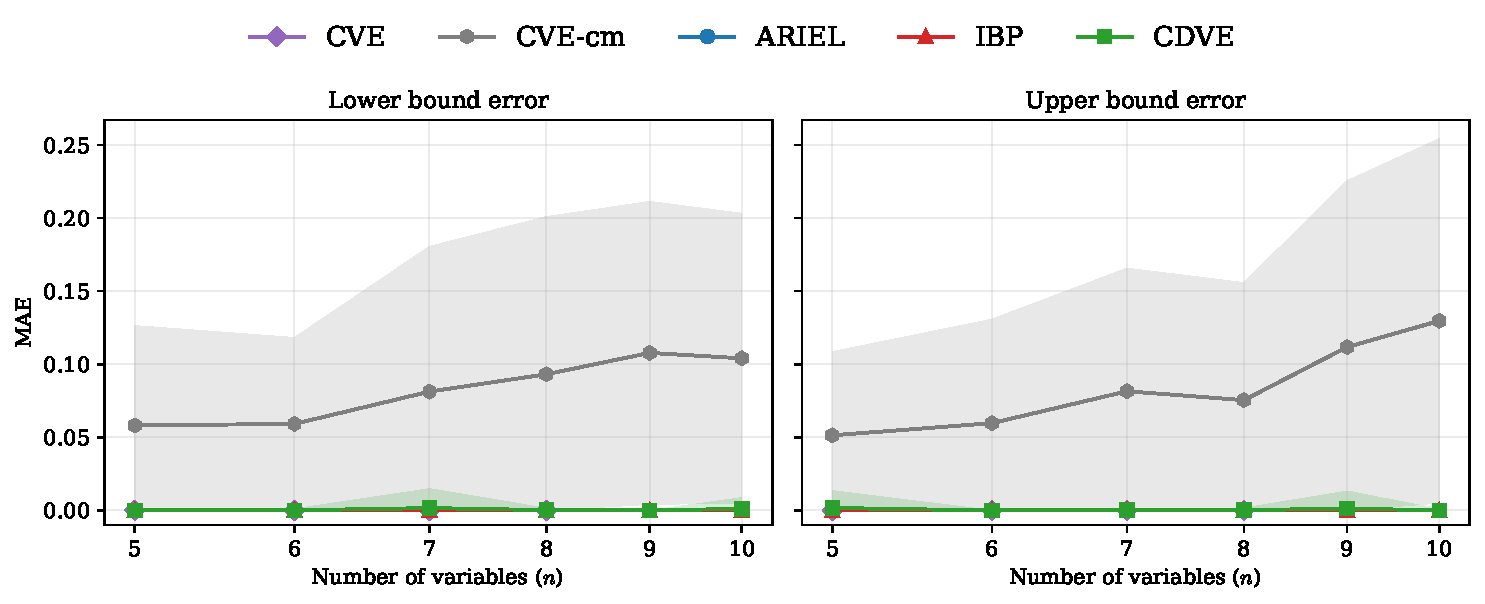
\includegraphics[width=\linewidth]{tree_small_fr_mae.pdf}
        \caption{small, error}
    \end{subfigure}\hfill
    \begin{subfigure}{0.49\linewidth}
        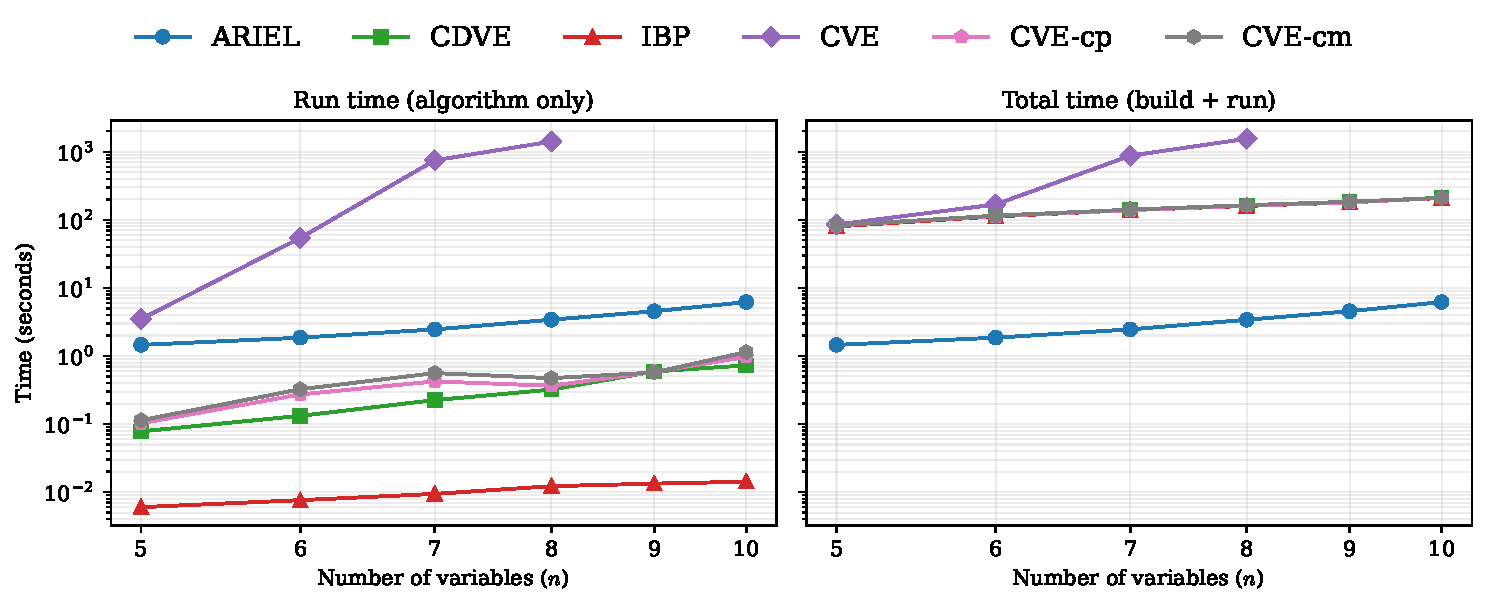
\includegraphics[width=\linewidth]{tree_small_fr_runtime.pdf}
        \caption{small, time}
    \end{subfigure}
    \\[0.3em]
    \begin{subfigure}{0.49\linewidth}
        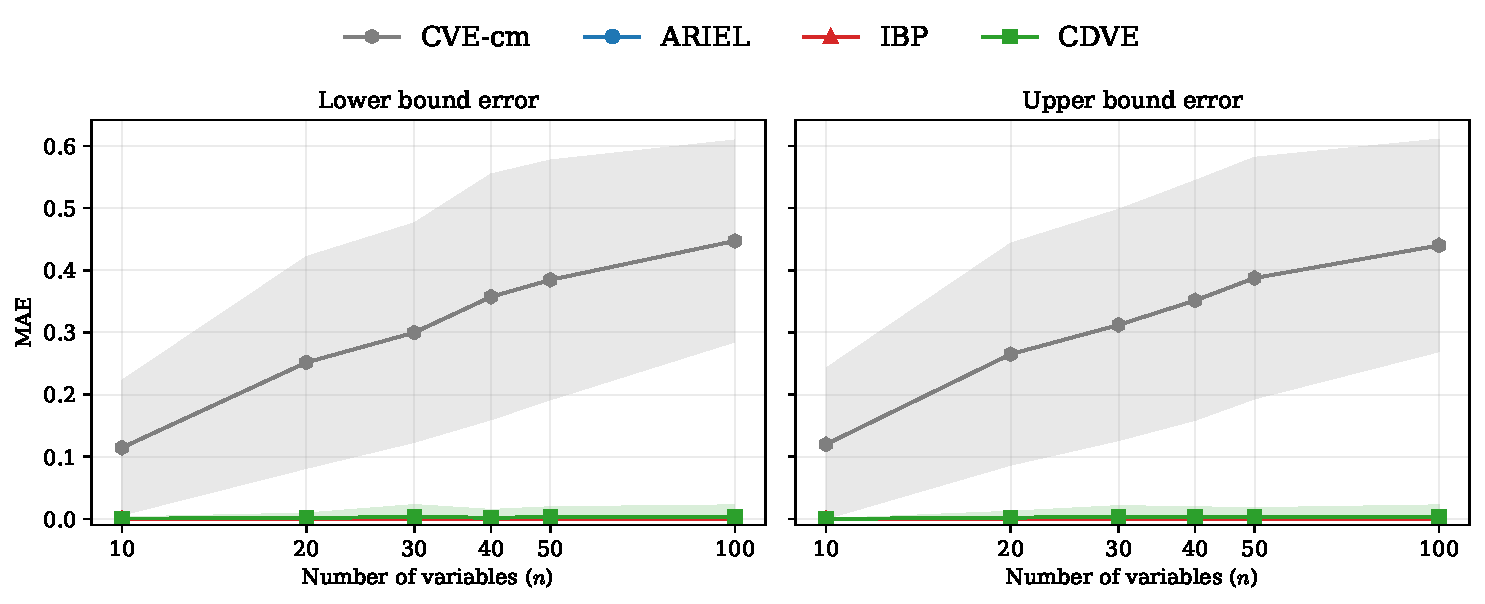
\includegraphics[width=\linewidth]{tree_large_fr_mae.pdf}
        \caption{large, error}
    \end{subfigure}\hfill
    \begin{subfigure}{0.49\linewidth}
        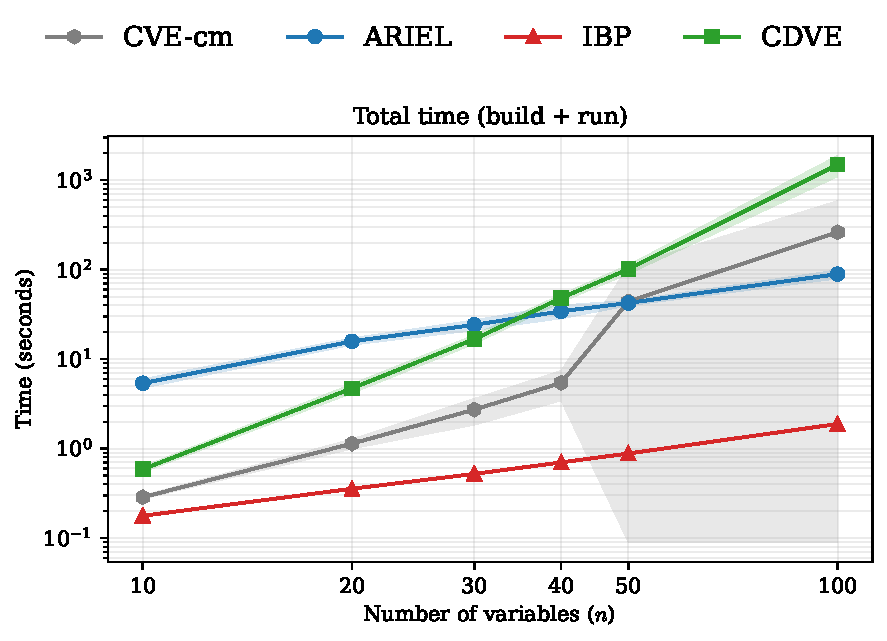
\includegraphics[width=\linewidth]{tree_large_fr_runtime.pdf}
        \caption{large, time}
    \end{subfigure}
    \caption{Random \texttt{tree} LCNs. Singly connected and fully realizable, so
    the credal-network relaxation is tight: ARIEL and IBP are indistinguishable
    from the reference.}
    \label{fig:tree-full}
\end{figure}

\begin{figure}[htbp]
    \centering
    \begin{subfigure}{0.49\linewidth}
        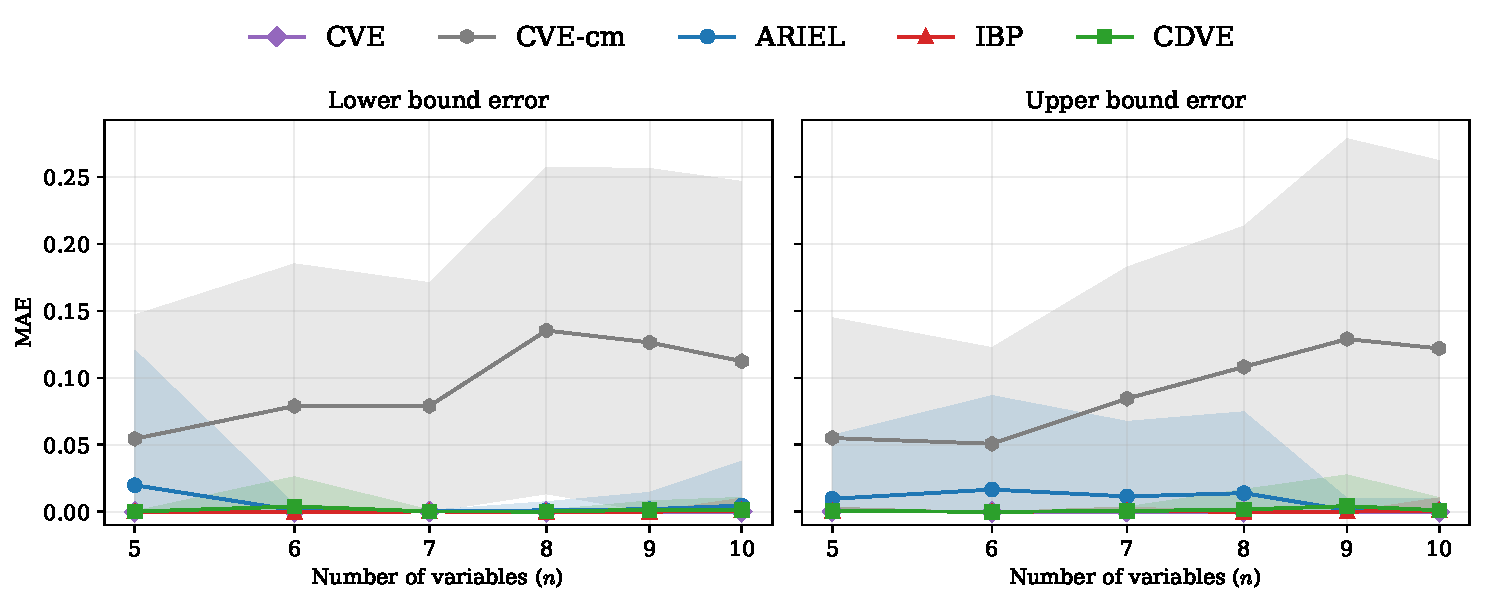
\includegraphics[width=\linewidth]{polytree_small_fr_mae.pdf}
        \caption{small, error}
    \end{subfigure}\hfill
    \begin{subfigure}{0.49\linewidth}
        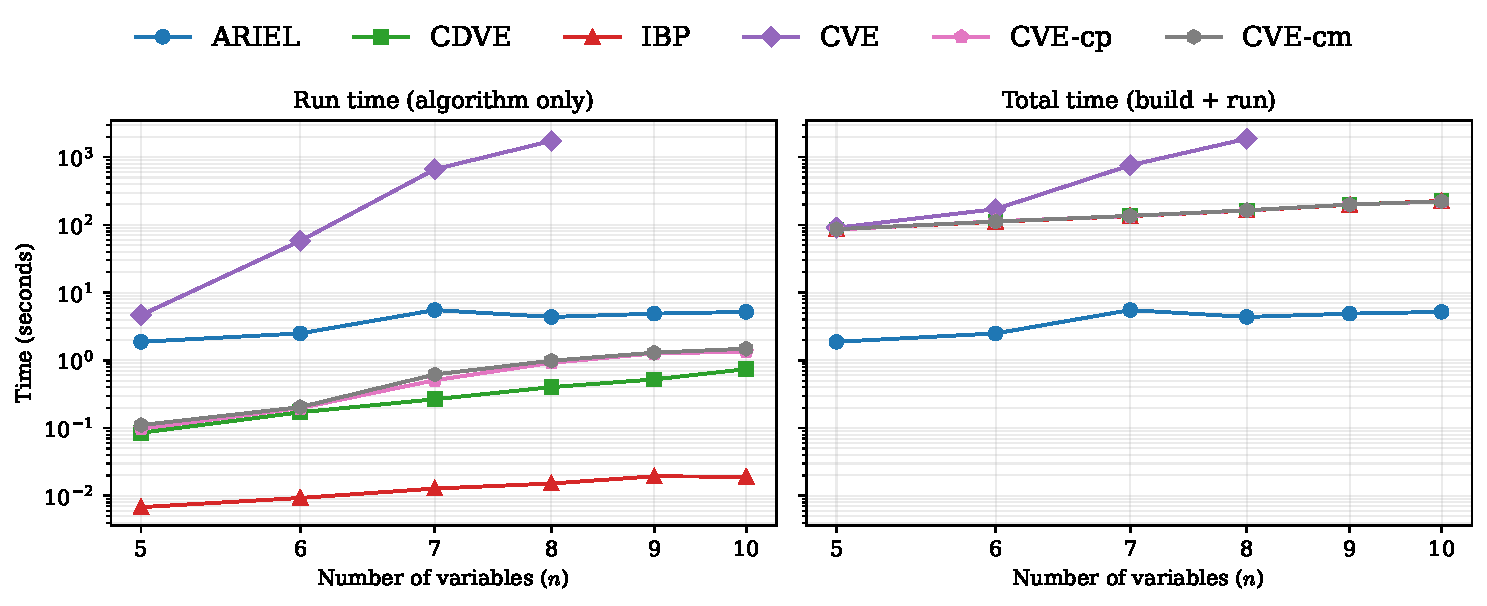
\includegraphics[width=\linewidth]{polytree_small_fr_runtime.pdf}
        \caption{small, time}
    \end{subfigure}
    \\[0.3em]
    \begin{subfigure}{0.49\linewidth}
        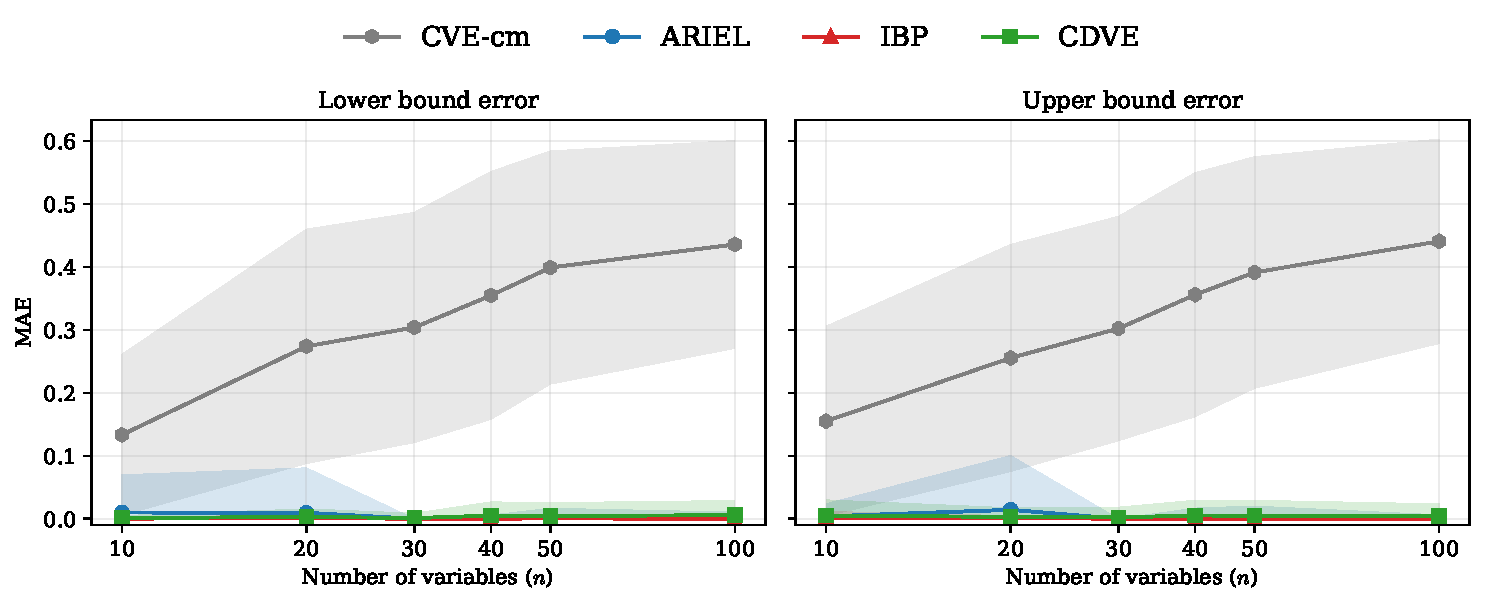
\includegraphics[width=\linewidth]{polytree_large_fr_mae.pdf}
        \caption{large, error}
    \end{subfigure}\hfill
    \begin{subfigure}{0.49\linewidth}
        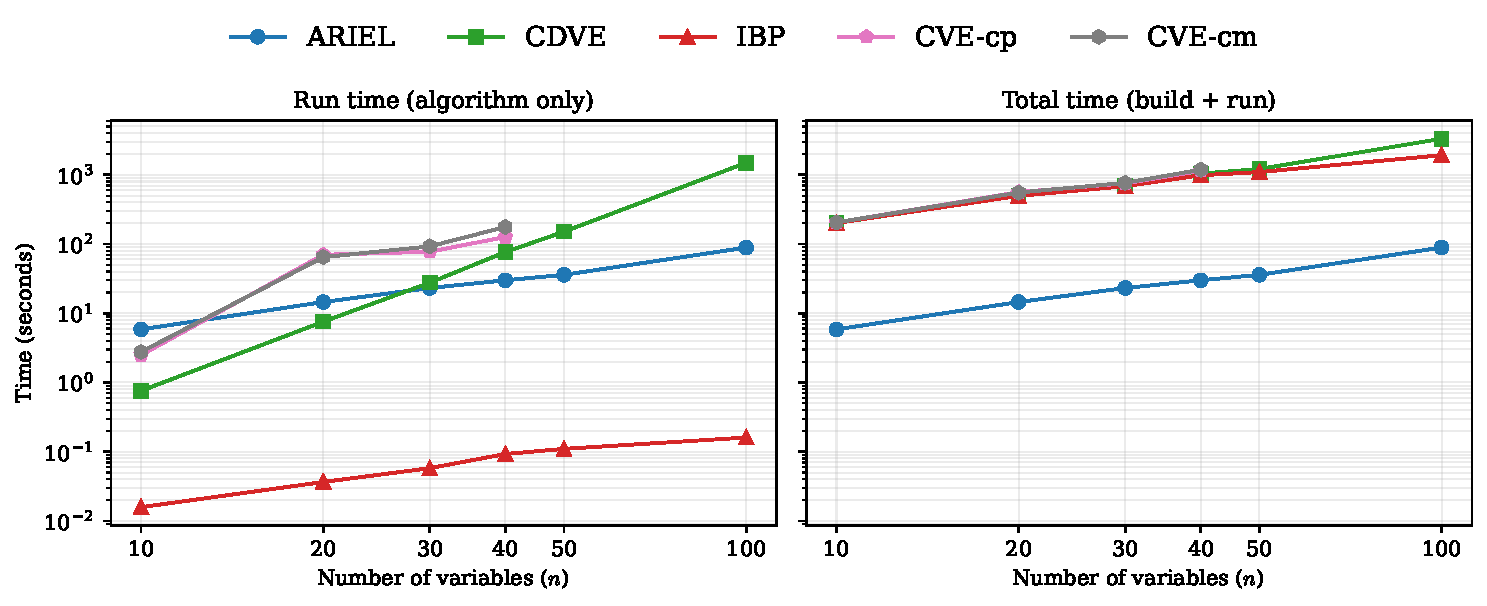
\includegraphics[width=\linewidth]{polytree_large_fr_runtime.pdf}
        \caption{large, time}
    \end{subfigure}
    \caption{Random \texttt{polytree} LCNs. Also singly connected; the residual
    ARIEL error at the small scale comes from instances where the reference
    itself is the tighter engine.}
    \label{fig:polytree-full}
\end{figure}

\begin{figure}[htbp]
    \centering
    \begin{subfigure}{0.49\linewidth}
        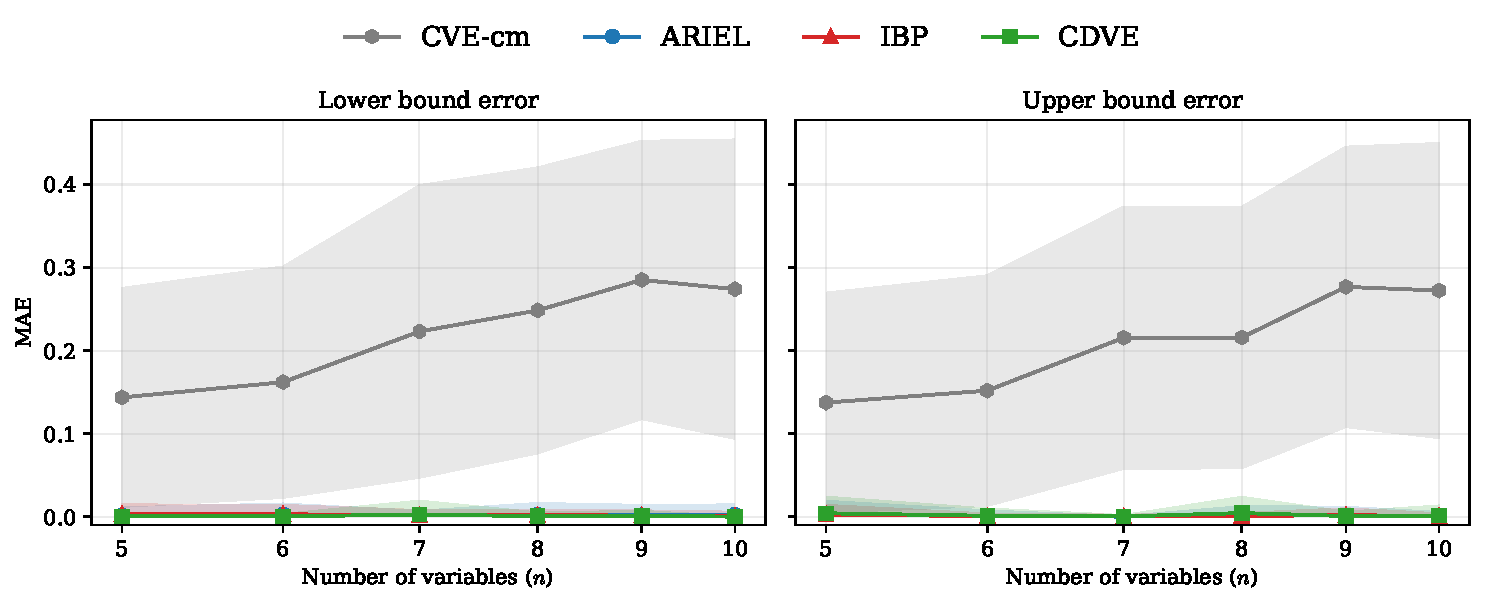
\includegraphics[width=\linewidth]{ktree_small_fr_mae.pdf}
        \caption{small, error}
    \end{subfigure}\hfill
    \begin{subfigure}{0.49\linewidth}
        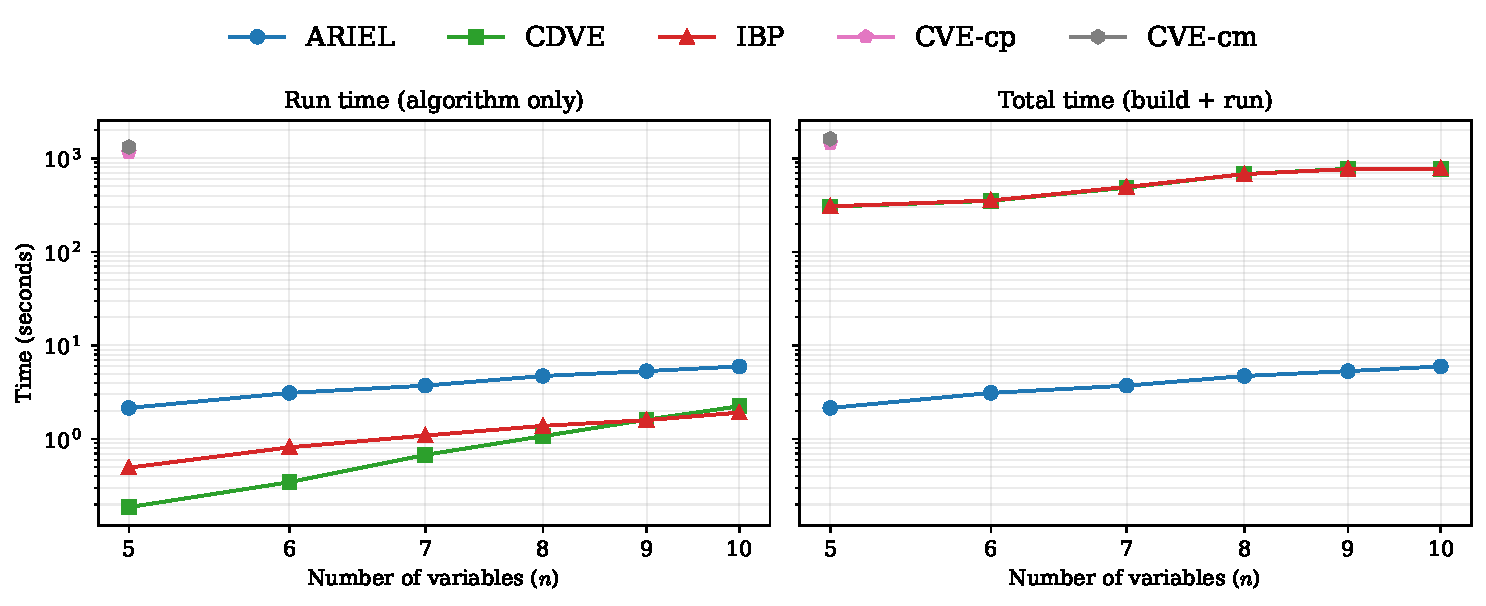
\includegraphics[width=\linewidth]{ktree_small_fr_runtime.pdf}
        \caption{small, time}
    \end{subfigure}
    \\[0.3em]
    \begin{subfigure}{0.49\linewidth}
        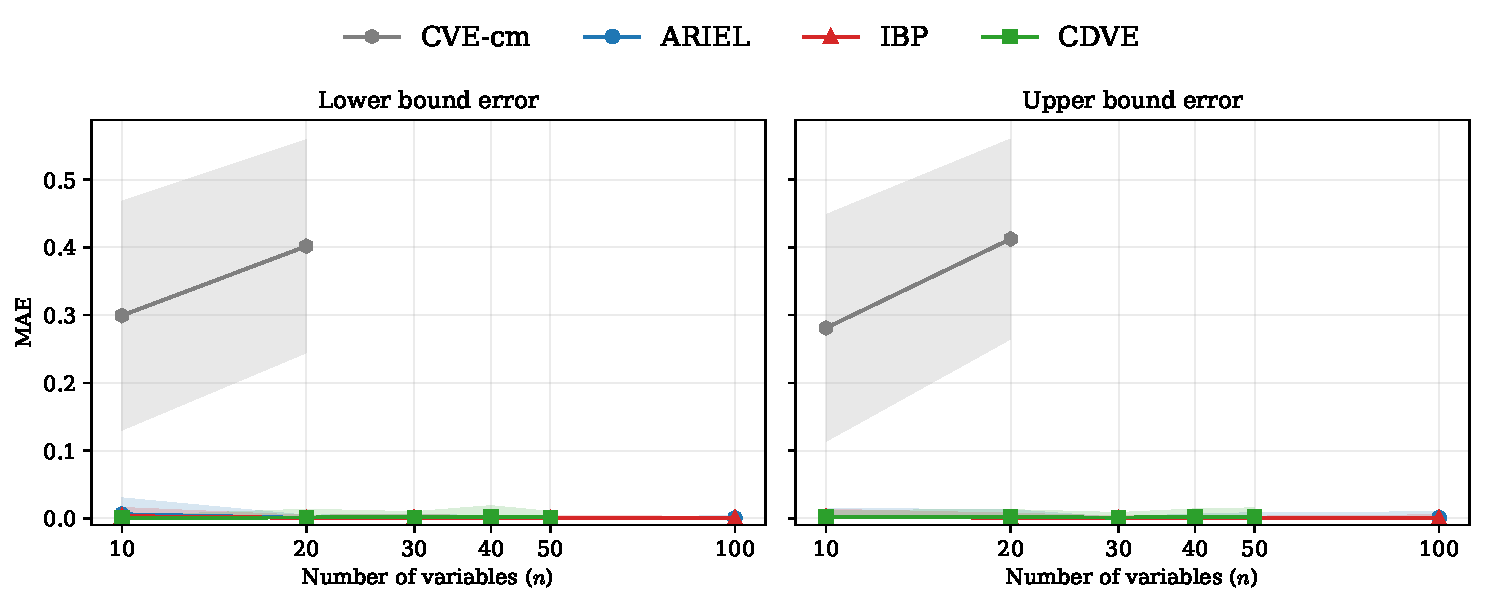
\includegraphics[width=\linewidth]{ktree_large_fr_mae.pdf}
        \caption{large, error}
    \end{subfigure}\hfill
    \begin{subfigure}{0.49\linewidth}
        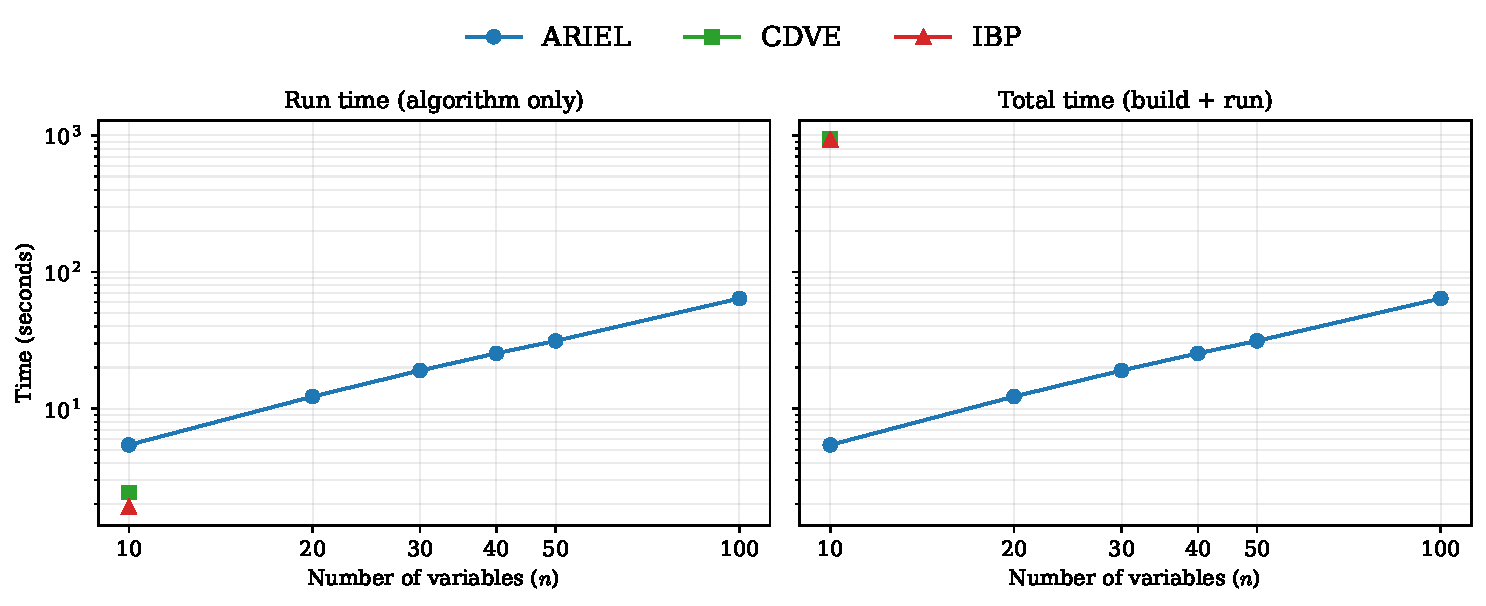
\includegraphics[width=\linewidth]{ktree_large_fr_runtime.pdf}
        \caption{large, time}
    \end{subfigure}
    \caption{Random \texttt{ktree} LCNs ($k{=}3$). Loopy despite bounded
    treewidth, so all credal-network methods give outer bounds only; plain CVE
    solves none of these instances and CVE$_{cm}$ stops after $n{=}20$.}
    \label{fig:ktree-full}
\end{figure}

\begin{figure}[htbp]
    \centering
    \begin{subfigure}{0.49\linewidth}
        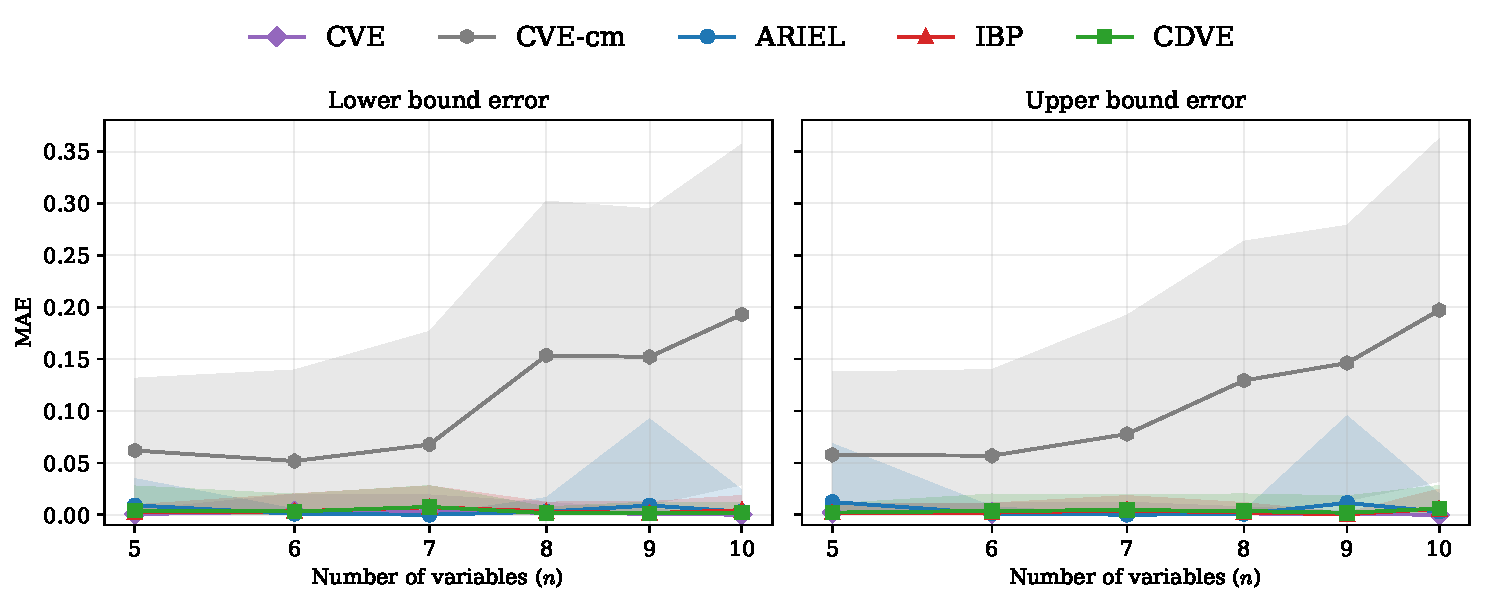
\includegraphics[width=\linewidth]{dag_small_fr_mae.pdf}
        \caption{small, error}
    \end{subfigure}\hfill
    \begin{subfigure}{0.49\linewidth}
        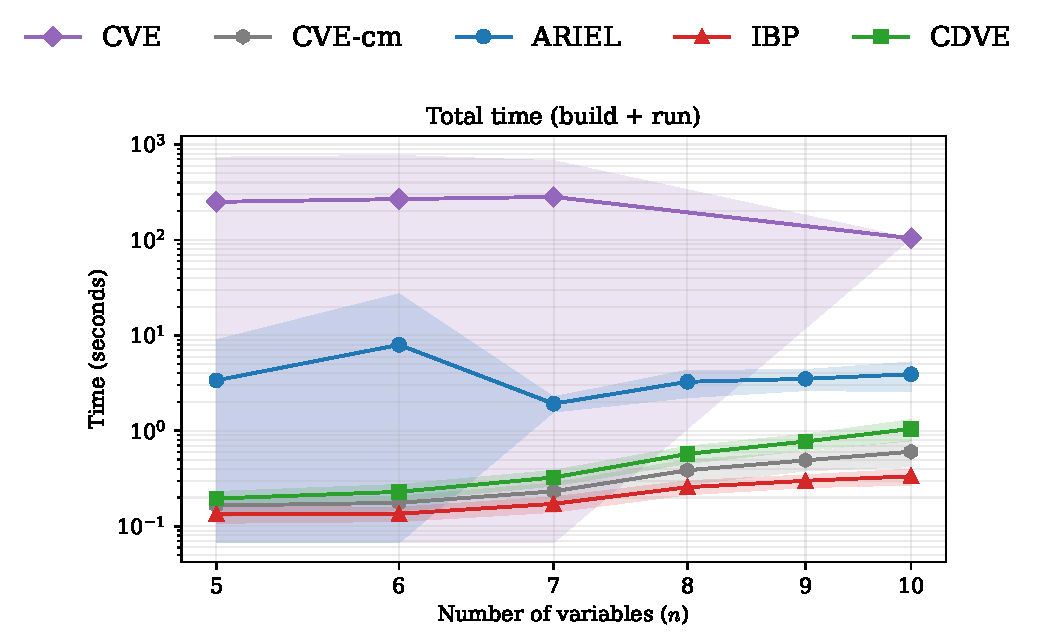
\includegraphics[width=\linewidth]{dag_small_fr_runtime.pdf}
        \caption{small, time}
    \end{subfigure}
    \\[0.3em]
    \begin{subfigure}{0.49\linewidth}
        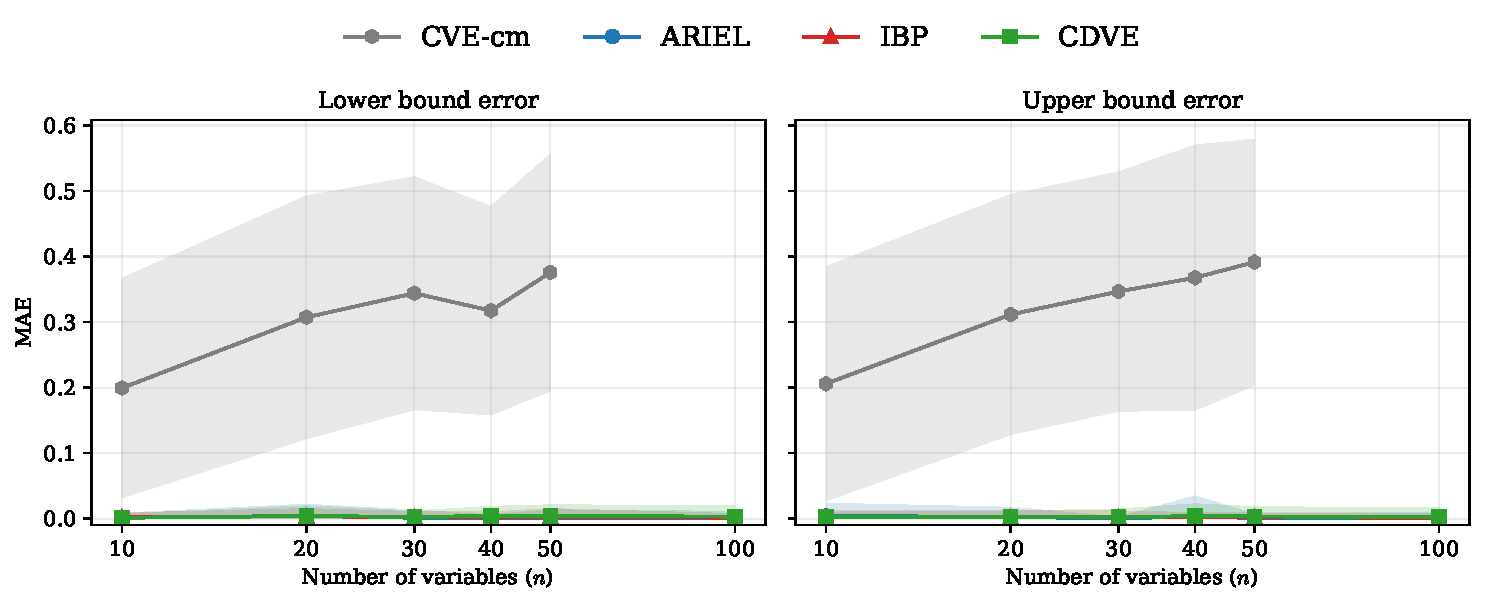
\includegraphics[width=\linewidth]{dag_large_fr_mae.pdf}
        \caption{large, error}
    \end{subfigure}\hfill
    \begin{subfigure}{0.49\linewidth}
        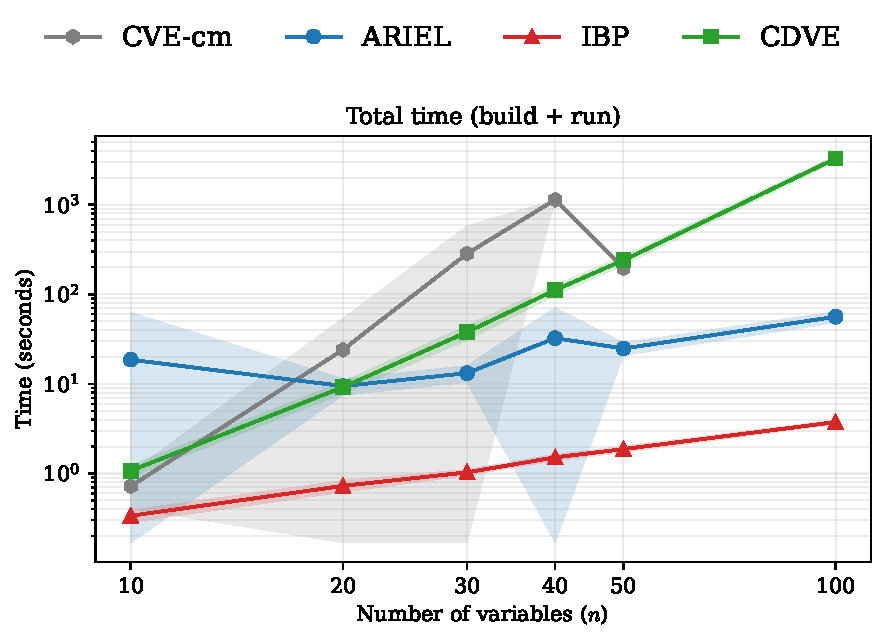
\includegraphics[width=\linewidth]{dag_large_fr_runtime.pdf}
        \caption{large, time}
    \end{subfigure}
    \caption{Random \texttt{dag} LCNs (moralized treewidth $\le 3$, at most two
    parents). The least structured family; CDVE's runtime grows fastest here,
    exceeding $600$ seconds at $n{=}100$.}
    \label{fig:dag-full}
\end{figure}

\clearpage
\begin{table}[ht]
\centering
\scriptsize
\caption{Error metrics vs.\ cjt reference}
\begin{tabular}{lrlrrrrrrr}
\toprule
Type & $n$ & Algorithm & MAE$_{\text{lb}}$ & MAE$_{\text{ub}}$ & Build & Run & Total & Ref & IW \\
\midrule
-- & 5 & approxlp & 0.0001 & 0.0017 & 80.42 & 0.08 & 80.49 & 0.31 & 1.00 \\
-- & 5 & ariel & 0.0000 & 0.0000 & 0.00 & 1.45 & 1.45 & 0.31 & -- \\
-- & 5 & cve & 0.0000 & 0.0000 & 81.83 & 3.48 & 85.31 & 0.31 & 1.00 \\
-- & 5 & $\text{cve\_cm}$ & 0.0426 & 0.0495 & 82.87 & 0.11 & 82.98 & 0.31 & 1.00 \\
-- & 5 & $\text{cve\_cp}$ & 0.1373 & 0.1438 & 82.37 & 0.10 & 82.47 & 0.31 & 1.00 \\
-- & 5 & ibp & 0.0000 & 0.0000 & 80.13 & 0.01 & 80.14 & 0.31 & 1.00 \\
-- & 6 & approxlp & 0.0001 & 0.0000 & 114.97 & 0.13 & 115.11 & 0.28 & 1.00 \\
-- & 6 & ariel & 0.0000 & 0.0000 & 0.00 & 1.86 & 1.86 & 0.28 & -- \\
-- & 6 & cve & 0.0000 & 0.0000 & 114.36 & 54.20 & 168.56 & 0.28 & 1.00 \\
-- & 6 & $\text{cve\_cm}$ & 0.0537 & 0.0511 & 115.02 & 0.32 & 115.34 & 0.28 & 1.00 \\
-- & 6 & $\text{cve\_cp}$ & 0.1930 & 0.1817 & 114.07 & 0.27 & 114.34 & 0.28 & 1.00 \\
-- & 6 & ibp & 0.0000 & 0.0000 & 112.40 & 0.01 & 112.40 & 0.28 & 1.00 \\
-- & 7 & approxlp & 0.0016 & 0.0002 & 138.66 & 0.22 & 138.88 & 0.33 & 1.00 \\
-- & 7 & ariel & 0.0000 & 0.0000 & 0.00 & 2.46 & 2.46 & 0.33 & -- \\
-- & 7 & cve & 0.0000 & 0.0000 & 126.08 & 751.00 & 877.07 & 0.33 & 1.00 \\
-- & 7 & $\text{cve\_cm}$ & 0.0697 & 0.0637 & 140.72 & 0.56 & 141.28 & 0.33 & 1.00 \\
-- & 7 & $\text{cve\_cp}$ & 0.2125 & 0.2135 & 138.42 & 0.42 & 138.84 & 0.33 & 1.00 \\
-- & 7 & ibp & 0.0000 & 0.0000 & 139.07 & 0.01 & 139.08 & 0.33 & 1.00 \\
-- & 8 & approxlp & 0.0002 & 0.0002 & 161.80 & 0.32 & 162.12 & 0.39 & 1.00 \\
-- & 8 & ariel & 0.0000 & 0.0000 & 0.00 & 3.41 & 3.41 & 0.39 & -- \\
-- & 8 & cve & 0.0000 & 0.0000 & 140.85 & 1415.83 & 1556.68 & 0.39 & 1.00 \\
-- & 8 & $\text{cve\_cm}$ & 0.0787 & 0.0704 & 163.92 & 0.47 & 164.39 & 0.39 & 1.00 \\
-- & 8 & $\text{cve\_cp}$ & 0.2142 & 0.2084 & 161.34 & 0.36 & 161.71 & 0.39 & 1.00 \\
-- & 8 & ibp & 0.0000 & 0.0000 & 160.44 & 0.01 & 160.46 & 0.39 & 1.00 \\
-- & 9 & approxlp & 0.0000 & 0.0013 & 181.78 & 0.59 & 182.37 & 0.44 & 1.00 \\
-- & 9 & ariel & 0.0000 & 0.0000 & 0.00 & 4.55 & 4.55 & 0.44 & -- \\
-- & 9 & $\text{cve\_cm}$ & 0.0860 & 0.1000 & 184.07 & 0.57 & 184.64 & 0.44 & 1.00 \\
-- & 9 & $\text{cve\_cp}$ & 0.2373 & 0.2458 & 180.04 & 0.58 & 180.63 & 0.44 & 1.00 \\
-- & 9 & ibp & 0.0000 & 0.0000 & 180.64 & 0.01 & 180.66 & 0.44 & 1.00 \\
-- & 10 & approxlp & 0.0011 & 0.0001 & 211.15 & 0.73 & 211.88 & 0.50 & 1.00 \\
-- & 10 & ariel & 0.0000 & 0.0000 & 0.00 & 6.19 & 6.19 & 0.50 & -- \\
-- & 10 & $\text{cve\_cm}$ & 0.0845 & 0.1065 & 209.71 & 1.14 & 210.85 & 0.50 & 1.00 \\
-- & 10 & $\text{cve\_cp}$ & 0.2641 & 0.2689 & 210.34 & 0.97 & 211.31 & 0.50 & 1.00 \\
-- & 10 & ibp & 0.0000 & 0.0000 & 210.06 & 0.01 & 210.08 & 0.50 & 1.00 \\
\bottomrule
\end{tabular}
\end{table}

\begin{table}[ht]
\centering
\scriptsize
\caption{Mean error metrics vs.\ CJT reference}
\begin{tabular}{lrlrrrrrrr}
\toprule
Type & $n$ & Algorithm & MAE$_{\text{lb}}$ & MAE$_{\text{ub}}$ & Build & Run & Total & Ref & IW \\
\midrule
$\text{tree\_fr}$ & 10 & CDVE & 0.0005 & 0.0000 & 0.18 & 0.41 & 0.59 & 0.64 & 1.00 \\
$\text{tree\_fr}$ & 10 & ARIEL & 0.0000 & 0.0000 & 0.00 & 5.37 & 5.37 & 0.64 & -- \\
$\text{tree\_fr}$ & 10 & CVE$_{cm}$ & 0.1145 & 0.1199 & 0.18 & 0.11 & 0.29 & 0.64 & 1.00 \\
$\text{tree\_fr}$ & 10 & IBP & 0.0000 & 0.0000 & 0.17 & 0.01 & 0.18 & 0.64 & 1.00 \\
\hline
$\text{tree\_fr}$ & 20 & CDVE & 0.0011 & 0.0019 & 0.35 & 4.36 & 4.71 & 1.43 & 1.00 \\
$\text{tree\_fr}$ & 20 & ARIEL & 0.0000 & 0.0000 & 0.00 & 15.80 & 15.80 & 1.43 & -- \\
$\text{tree\_fr}$ & 20 & CVE$_{cm}$ & 0.2517 & 0.2650 & 0.37 & 0.77 & 1.14 & 1.43 & 1.00 \\
$\text{tree\_fr}$ & 20 & IBP & 0.0000 & 0.0000 & 0.34 & 0.02 & 0.36 & 1.43 & 1.00 \\
\hline
$\text{tree\_fr}$ & 30 & CDVE & 0.0036 & 0.0037 & 0.50 & 16.18 & 16.68 & 2.58 & 1.00 \\
$\text{tree\_fr}$ & 30 & ARIEL & 0.0000 & 0.0000 & 0.00 & 24.13 & 24.13 & 2.58 & -- \\
$\text{tree\_fr}$ & 30 & CVE$_{cm}$ & 0.2998 & 0.3120 & 0.55 & 2.18 & 2.73 & 2.58 & 1.00 \\
$\text{tree\_fr}$ & 30 & IBP & 0.0000 & 0.0000 & 0.49 & 0.03 & 0.52 & 2.58 & 1.00 \\
\hline
$\text{tree\_fr}$ & 40 & CDVE & 0.0017 & 0.0026 & 0.66 & 47.39 & 48.04 & 3.90 & 1.00 \\
$\text{tree\_fr}$ & 40 & ARIEL & 0.0000 & 0.0000 & 0.00 & 34.21 & 34.21 & 3.90 & -- \\
$\text{tree\_fr}$ & 40 & CVE$_{cm}$ & 0.3573 & 0.3515 & 0.70 & 4.72 & 5.43 & 3.90 & 1.00 \\
$\text{tree\_fr}$ & 40 & IBP & 0.0000 & 0.0000 & 0.66 & 0.04 & 0.70 & 3.90 & 1.00 \\
\hline
$\text{tree\_fr}$ & 50 & CDVE & 0.0031 & 0.0026 & 0.83 & 100.39 & 101.22 & 5.95 & 1.00 \\
$\text{tree\_fr}$ & 50 & ARIEL & 0.0000 & 0.0000 & 0.00 & 42.41 & 42.41 & 5.95 & -- \\
$\text{tree\_fr}$ & 50 & CVE$_{cm}$ & 0.3845 & 0.3875 & 0.96 & 43.09 & 44.05 & 5.95 & 1.00 \\
$\text{tree\_fr}$ & 50 & IBP & 0.0000 & 0.0000 & 0.83 & 0.05 & 0.88 & 5.95 & 1.00 \\
\hline
$\text{tree\_fr}$ & 100 & CDVE & 0.0037 & 0.0036 & 1.67 & 1487.61 & 1489.29 & 16.24 & 1.00 \\
$\text{tree\_fr}$ & 100 & ARIEL & 0.0000 & 0.0000 & 0.00 & 89.09 & 89.09 & 16.24 & -- \\
$\text{tree\_fr}$ & 100 & CVE$_{cm}$ & 0.4473 & 0.4401 & 1.94 & 259.37 & 261.31 & 16.24 & 1.00 \\
$\text{tree\_fr}$ & 100 & IBP & 0.0000 & 0.0000 & 1.76 & 0.12 & 1.88 & 16.24 & 1.00 \\
\bottomrule
\end{tabular}
\end{table}

\begin{table}[ht]
\centering
\scriptsize
\caption{Standard deviation of error metrics vs.\ CJT reference}
\begin{tabular}{lrlrrrrrrr}
\toprule
Type & $n$ & Algorithm & SD$_{\text{lb}}$ & SD$_{\text{ub}}$ & Build & Run & Total & Ref & IW \\
\midrule
$\text{tree\_fr}$ & 10 & CDVE & 0.0026 & 0.0003 & 0.18 & 0.41 & 0.59 & 0.64 & 1.00 \\
$\text{tree\_fr}$ & 10 & ARIEL & 0.0000 & 0.0000 & 0.00 & 5.37 & 5.37 & 0.64 & -- \\
$\text{tree\_fr}$ & 10 & CVE$_{cm}$ & 0.1085 & 0.1227 & 0.18 & 0.11 & 0.29 & 0.64 & 1.00 \\
$\text{tree\_fr}$ & 10 & IBP & 0.0000 & 0.0000 & 0.17 & 0.01 & 0.18 & 0.64 & 1.00 \\
\hline
$\text{tree\_fr}$ & 20 & CDVE & 0.0083 & 0.0104 & 0.35 & 4.36 & 4.71 & 1.43 & 1.00 \\
$\text{tree\_fr}$ & 20 & ARIEL & 0.0000 & 0.0000 & 0.00 & 15.80 & 15.80 & 1.43 & -- \\
$\text{tree\_fr}$ & 20 & CVE$_{cm}$ & 0.1704 & 0.1786 & 0.37 & 0.77 & 1.14 & 1.43 & 1.00 \\
$\text{tree\_fr}$ & 20 & IBP & 0.0000 & 0.0000 & 0.34 & 0.02 & 0.36 & 1.43 & 1.00 \\
\hline
$\text{tree\_fr}$ & 30 & CDVE & 0.0195 & 0.0177 & 0.50 & 16.18 & 16.68 & 2.58 & 1.00 \\
$\text{tree\_fr}$ & 30 & ARIEL & 0.0000 & 0.0000 & 0.00 & 24.13 & 24.13 & 2.58 & -- \\
$\text{tree\_fr}$ & 30 & CVE$_{cm}$ & 0.1766 & 0.1860 & 0.55 & 2.18 & 2.73 & 2.58 & 1.00 \\
$\text{tree\_fr}$ & 30 & IBP & 0.0000 & 0.0000 & 0.49 & 0.03 & 0.52 & 2.58 & 1.00 \\
\hline
$\text{tree\_fr}$ & 40 & CDVE & 0.0134 & 0.0169 & 0.66 & 47.39 & 48.04 & 3.90 & 1.00 \\
$\text{tree\_fr}$ & 40 & ARIEL & 0.0000 & 0.0000 & 0.00 & 34.21 & 34.21 & 3.90 & -- \\
$\text{tree\_fr}$ & 40 & CVE$_{cm}$ & 0.1977 & 0.1929 & 0.70 & 4.72 & 5.43 & 3.90 & 1.00 \\
$\text{tree\_fr}$ & 40 & IBP & 0.0000 & 0.0000 & 0.66 & 0.04 & 0.70 & 3.90 & 1.00 \\
\hline
$\text{tree\_fr}$ & 50 & CDVE & 0.0164 & 0.0154 & 0.83 & 100.39 & 101.22 & 5.95 & 1.00 \\
$\text{tree\_fr}$ & 50 & ARIEL & 0.0000 & 0.0000 & 0.00 & 42.41 & 42.41 & 5.95 & -- \\
$\text{tree\_fr}$ & 50 & CVE$_{cm}$ & 0.1929 & 0.1944 & 0.96 & 43.09 & 44.05 & 5.95 & 1.00 \\
$\text{tree\_fr}$ & 50 & IBP & 0.0000 & 0.0000 & 0.83 & 0.05 & 0.88 & 5.95 & 1.00 \\
\hline
$\text{tree\_fr}$ & 100 & CDVE & 0.0189 & 0.0190 & 1.67 & 1487.61 & 1489.29 & 16.24 & 1.00 \\
$\text{tree\_fr}$ & 100 & ARIEL & 0.0000 & 0.0000 & 0.00 & 89.09 & 89.09 & 16.24 & -- \\
$\text{tree\_fr}$ & 100 & CVE$_{cm}$ & 0.1625 & 0.1711 & 1.94 & 259.37 & 261.31 & 16.24 & 1.00 \\
$\text{tree\_fr}$ & 100 & IBP & 0.0000 & 0.0000 & 1.76 & 0.12 & 1.88 & 16.24 & 1.00 \\
\bottomrule
\end{tabular}
\end{table}

\clearpage
\begin{table}[ht]
\centering
\scriptsize
\caption{Error metrics vs.\ cjt reference}
\begin{tabular}{lrlrrrrrrr}
\toprule
Type & $n$ & Algorithm & MAE$_{\text{lb}}$ & MAE$_{\text{ub}}$ & Build & Run & Total & Ref & IW \\
\midrule
-- & 5 & approxlp & 0.0053 & 0.0041 & 85.64 & 0.09 & 85.72 & 0.80 & 1.20 \\
-- & 5 & ariel & 0.0050 & 0.0135 & 0.00 & 1.88 & 1.88 & 0.80 & -- \\
-- & 5 & cve & 0.0051 & 0.0041 & 85.92 & 4.66 & 90.57 & 0.80 & 1.20 \\
-- & 5 & $\text{cve\_cm}$ & 0.0375 & 0.0483 & 86.23 & 0.11 & 86.34 & 0.80 & 1.20 \\
-- & 5 & $\text{cve\_cp}$ & 0.1179 & 0.1508 & 85.12 & 0.10 & 85.22 & 0.80 & 1.20 \\
-- & 5 & ibp & 0.0051 & 0.0041 & 85.70 & 0.01 & 85.71 & 0.80 & 1.20 \\
-- & 6 & approxlp & 0.0000 & 0.0009 & 111.45 & 0.17 & 111.62 & 0.36 & 1.22 \\
-- & 6 & ariel & 0.0000 & 0.0000 & 0.00 & 2.50 & 2.50 & 0.36 & -- \\
-- & 6 & cve & 0.0000 & 0.0001 & 112.91 & 57.96 & 170.87 & 0.36 & 1.22 \\
-- & 6 & $\text{cve\_cm}$ & 0.0531 & 0.0482 & 111.84 & 0.20 & 112.05 & 0.36 & 1.22 \\
-- & 6 & $\text{cve\_cp}$ & 0.1601 & 0.1468 & 112.66 & 0.20 & 112.86 & 0.36 & 1.22 \\
-- & 6 & ibp & 0.0000 & 0.0001 & 111.24 & 0.01 & 111.25 & 0.36 & 1.22 \\
-- & 7 & approxlp & 0.0003 & 0.0071 & 134.97 & 0.27 & 135.24 & 0.58 & 1.33 \\
-- & 7 & ariel & 0.0000 & 0.0000 & 0.00 & 5.52 & 5.52 & 0.58 & -- \\
-- & 7 & cve & 0.0000 & 0.0000 & 96.79 & 661.68 & 758.47 & 0.58 & 1.25 \\
-- & 7 & $\text{cve\_cm}$ & 0.0620 & 0.0751 & 135.27 & 0.62 & 135.88 & 0.58 & 1.33 \\
-- & 7 & $\text{cve\_cp}$ & 0.1759 & 0.1881 & 134.66 & 0.51 & 135.17 & 0.58 & 1.33 \\
-- & 7 & ibp & 0.0002 & 0.0068 & 134.51 & 0.01 & 134.52 & 0.58 & 1.33 \\
-- & 8 & approxlp & 0.0016 & 0.0018 & 162.95 & 0.40 & 163.35 & 95.97 & 1.30 \\
-- & 8 & ariel & 0.0019 & 0.0002 & 0.00 & 4.37 & 4.37 & 95.97 & -- \\
-- & 8 & cve & 0.0000 & 0.0000 & 133.93 & 1733.25 & 1867.19 & 95.97 & 1.00 \\
-- & 8 & $\text{cve\_cm}$ & 0.0918 & 0.0815 & 163.05 & 0.99 & 164.04 & 95.97 & 1.30 \\
-- & 8 & $\text{cve\_cp}$ & 0.2224 & 0.2236 & 162.34 & 0.92 & 163.26 & 95.97 & 1.30 \\
-- & 8 & ibp & 0.0016 & 0.0000 & 162.17 & 0.02 & 162.19 & 95.97 & 1.30 \\
-- & 9 & approxlp & 0.0058 & 0.0068 & 198.50 & 0.52 & 199.03 & 0.66 & 1.50 \\
-- & 9 & ariel & 0.0000 & 0.0000 & 0.00 & 4.89 & 4.89 & 0.66 & -- \\
-- & 9 & $\text{cve\_cm}$ & 0.1022 & 0.1045 & 198.03 & 1.30 & 199.33 & 0.66 & 1.50 \\
-- & 9 & $\text{cve\_cp}$ & 0.2492 & 0.2527 & 198.42 & 1.27 & 199.68 & 0.66 & 1.50 \\
-- & 9 & ibp & 0.0054 & 0.0038 & 198.24 & 0.02 & 198.26 & 0.66 & 1.50 \\
-- & 10 & approxlp & 0.0103 & 0.0035 & 223.76 & 0.74 & 224.50 & 1.08 & 1.56 \\
-- & 10 & ariel & 0.0021 & 0.0007 & 0.00 & 5.19 & 5.19 & 1.08 & -- \\
-- & 10 & $\text{cve\_cm}$ & 0.0847 & 0.0973 & 220.77 & 1.49 & 222.25 & 1.08 & 1.56 \\
-- & 10 & $\text{cve\_cp}$ & 0.2396 & 0.2599 & 220.02 & 1.34 & 221.36 & 1.08 & 1.56 \\
-- & 10 & ibp & 0.0079 & 0.0031 & 225.34 & 0.02 & 225.36 & 1.08 & 1.56 \\
\bottomrule
\end{tabular}
\end{table}

\begin{table}[ht]
\centering
\scriptsize
\caption{Error metrics vs.\ cjt reference}
\begin{tabular}{lrlrrrrrrr}
\toprule
Type & $n$ & Algorithm & MAE$_{\text{lb}}$ & MAE$_{\text{ub}}$ & Build & Run & Total & Ref & IW \\
\midrule
-- & 10 & approxlp & 0.0018 & 0.0018 & 199.93 & 0.76 & 200.69 & 0.51 & 1.10 \\
-- & 10 & ariel & 0.0000 & 0.0000 & 0.00 & 5.84 & 5.84 & 0.51 & -- \\
-- & 10 & $\text{cve\_cm}$ & 0.0772 & 0.0923 & 201.91 & 2.76 & 204.67 & 0.51 & 1.10 \\
-- & 10 & $\text{cve\_cp}$ & 0.2174 & 0.2262 & 201.58 & 2.49 & 204.07 & 0.51 & 1.10 \\
-- & 10 & ibp & 0.0016 & 0.0000 & 201.27 & 0.02 & 201.29 & 0.51 & 1.10 \\
-- & 20 & approxlp & 0.0032 & 0.0052 & 490.42 & 7.55 & 497.97 & 1.68 & 1.50 \\
-- & 20 & ariel & 0.0000 & 0.0000 & 0.00 & 14.52 & 14.52 & 1.68 & -- \\
-- & 20 & $\text{cve\_cm}$ & 0.2155 & 0.2224 & 489.09 & 64.64 & 553.73 & 1.68 & 1.50 \\
-- & 20 & $\text{cve\_cp}$ & 0.3322 & 0.3285 & 491.70 & 69.90 & 561.60 & 1.68 & 1.50 \\
-- & 20 & ibp & 0.0030 & 0.0021 & 496.49 & 0.04 & 496.53 & 1.68 & 1.50 \\
-- & 30 & approxlp & 0.0018 & 0.0030 & 672.72 & 27.61 & 700.33 & 2.60 & 1.20 \\
-- & 30 & ariel & 0.0000 & 0.0000 & 0.00 & 23.15 & 23.15 & 2.60 & -- \\
-- & 30 & $\text{cve\_cm}$ & 0.2733 & 0.2938 & 671.86 & 92.44 & 764.30 & 2.60 & 1.20 \\
-- & 30 & $\text{cve\_cp}$ & 0.4186 & 0.3845 & 675.39 & 77.33 & 752.72 & 2.60 & 1.20 \\
-- & 30 & ibp & 0.0009 & 0.0008 & 683.33 & 0.06 & 683.39 & 2.60 & 1.20 \\
-- & 40 & approxlp & 0.0037 & 0.0059 & 961.90 & 76.60 & 1038.49 & 3.87 & 1.70 \\
-- & 40 & ariel & 0.0000 & 0.0000 & 0.00 & 29.93 & 29.93 & 3.87 & -- \\
-- & 40 & $\text{cve\_cm}$ & 0.3219 & 0.3139 & 1008.78 & 176.36 & 1185.13 & 3.87 & 2.00 \\
-- & 40 & $\text{cve\_cp}$ & 0.4213 & 0.3937 & 1012.33 & 126.60 & 1138.93 & 3.87 & 2.00 \\
-- & 40 & ibp & 0.0008 & 0.0026 & 985.06 & 0.09 & 985.15 & 3.87 & 1.70 \\
-- & 50 & approxlp & 0.0031 & 0.0066 & 1060.39 & 150.66 & 1211.05 & 5.31 & 1.80 \\
-- & 50 & ariel & 0.0000 & 0.0000 & 0.00 & 35.91 & 35.91 & 5.31 & -- \\
-- & 50 & ibp & 0.0008 & 0.0016 & 1094.34 & 0.11 & 1094.45 & 5.31 & 1.80 \\
-- & 100 & approxlp & 0.0058 & 0.0027 & 1825.88 & 1490.49 & 3316.37 & 14.44 & 1.17 \\
-- & 100 & ariel & 0.0000 & 0.0000 & 0.00 & 88.86 & 88.86 & 14.44 & -- \\
-- & 100 & ibp & 0.0014 & 0.0009 & 1919.66 & 0.16 & 1919.82 & 14.44 & 1.40 \\
\bottomrule
\end{tabular}
\end{table}

\clearpage
\begin{table}[ht]
\centering
\scriptsize
\caption{Mean error metrics vs.\ CJT reference}
\begin{tabular}{lrlrrrrrrr}
\toprule
Type & $n$ & Algorithm & MAE$_{\text{lb}}$ & MAE$_{\text{ub}}$ & Build & Run & Total & Ref & IW \\
\midrule
$\text{ktree\_fr\_k3}$ & 5 & CDVE & 0.0006 & 0.0042 & 0.33 & 0.14 & 0.48 & 0.29 & 3.00 \\
$\text{ktree\_fr\_k3}$ & 5 & ARIEL & 0.0015 & 0.0028 & 0.00 & 2.15 & 2.15 & 0.29 & -- \\
$\text{ktree\_fr\_k3}$ & 5 & CVE$_{cm}$ & 0.1437 & 0.1374 & 0.33 & 1.38 & 1.71 & 0.29 & 3.00 \\
$\text{ktree\_fr\_k3}$ & 5 & IBP & 0.0030 & 0.0027 & 0.33 & 0.41 & 0.74 & 0.29 & 3.00 \\
\hline
$\text{ktree\_fr\_k3}$ & 6 & CDVE & 0.0006 & 0.0012 & 0.45 & 0.29 & 0.74 & 0.36 & 3.00 \\
$\text{ktree\_fr\_k3}$ & 6 & ARIEL & 0.0029 & 0.0011 & 0.00 & 3.11 & 3.11 & 0.36 & -- \\
$\text{ktree\_fr\_k3}$ & 6 & CVE$_{cm}$ & 0.1620 & 0.1519 & 0.45 & 3.99 & 4.43 & 0.36 & 3.00 \\
$\text{ktree\_fr\_k3}$ & 6 & IBP & 0.0030 & 0.0008 & 0.45 & 0.69 & 1.14 & 0.36 & 3.00 \\
\hline
$\text{ktree\_fr\_k3}$ & 7 & CDVE & 0.0027 & 0.0005 & 0.57 & 0.59 & 1.17 & 0.42 & 3.00 \\
$\text{ktree\_fr\_k3}$ & 7 & ARIEL & 0.0015 & 0.0002 & 0.00 & 3.72 & 3.72 & 0.42 & -- \\
$\text{ktree\_fr\_k3}$ & 7 & CVE$_{cm}$ & 0.2231 & 0.2155 & 0.60 & 7.68 & 8.27 & 0.42 & 3.00 \\
$\text{ktree\_fr\_k3}$ & 7 & IBP & 0.0018 & 0.0005 & 0.58 & 0.92 & 1.50 & 0.42 & 3.00 \\
\hline
$\text{ktree\_fr\_k3}$ & 8 & CDVE & 0.0008 & 0.0044 & 0.64 & 0.90 & 1.54 & 0.51 & 3.00 \\
$\text{ktree\_fr\_k3}$ & 8 & ARIEL & 0.0028 & 0.0020 & 0.00 & 4.72 & 4.72 & 0.51 & -- \\
$\text{ktree\_fr\_k3}$ & 8 & CVE$_{cm}$ & 0.2484 & 0.2158 & 0.69 & 22.88 & 23.57 & 0.51 & 3.00 \\
$\text{ktree\_fr\_k3}$ & 8 & IBP & 0.0018 & 0.0011 & 0.71 & 1.23 & 1.94 & 0.51 & 3.00 \\
\hline
$\text{ktree\_fr\_k3}$ & 9 & CDVE & 0.0011 & 0.0009 & 0.78 & 1.39 & 2.17 & 0.60 & 3.00 \\
$\text{ktree\_fr\_k3}$ & 9 & ARIEL & 0.0019 & 0.0017 & 0.00 & 5.32 & 5.32 & 0.60 & -- \\
$\text{ktree\_fr\_k3}$ & 9 & CVE$_{cm}$ & 0.2851 & 0.2768 & 0.82 & 26.13 & 26.95 & 0.60 & 3.00 \\
$\text{ktree\_fr\_k3}$ & 9 & IBP & 0.0015 & 0.0020 & 0.76 & 1.38 & 2.13 & 0.60 & 3.00 \\
\hline
$\text{ktree\_fr\_k3}$ & 10 & CDVE & 0.0002 & 0.0015 & 0.95 & 2.10 & 3.05 & 0.68 & 3.00 \\
$\text{ktree\_fr\_k3}$ & 10 & ARIEL & 0.0027 & 0.0011 & 0.00 & 5.98 & 5.98 & 0.68 & -- \\
$\text{ktree\_fr\_k3}$ & 10 & CVE$_{cm}$ & 0.2740 & 0.2723 & 0.96 & 45.69 & 46.65 & 0.68 & 3.00 \\
$\text{ktree\_fr\_k3}$ & 10 & IBP & 0.0013 & 0.0009 & 0.97 & 1.74 & 2.70 & 0.68 & 3.00 \\
\bottomrule
\end{tabular}
\end{table}

\begin{table}[ht]
\centering
\scriptsize
\caption{Standard deviation of error metrics vs.\ CJT reference}
\begin{tabular}{lrlrrrrrrr}
\toprule
Type & $n$ & Algorithm & SD$_{\text{lb}}$ & SD$_{\text{ub}}$ & Build & Run & Total & Ref & IW \\
\midrule
$\text{ktree\_fr\_k3}$ & 5 & CDVE & 0.0021 & 0.0206 & 0.33 & 0.14 & 0.48 & 0.29 & 3.00 \\
$\text{ktree\_fr\_k3}$ & 5 & ARIEL & 0.0105 & 0.0171 & 0.00 & 2.15 & 2.15 & 0.29 & -- \\
$\text{ktree\_fr\_k3}$ & 5 & CVE$_{cm}$ & 0.1324 & 0.1330 & 0.33 & 1.38 & 1.71 & 0.29 & 3.00 \\
$\text{ktree\_fr\_k3}$ & 5 & IBP & 0.0125 & 0.0122 & 0.33 & 0.41 & 0.74 & 0.29 & 3.00 \\
\hline
$\text{ktree\_fr\_k3}$ & 6 & CDVE & 0.0034 & 0.0094 & 0.45 & 0.29 & 0.74 & 0.36 & 3.00 \\
$\text{ktree\_fr\_k3}$ & 6 & ARIEL & 0.0137 & 0.0071 & 0.00 & 3.11 & 3.11 & 0.36 & -- \\
$\text{ktree\_fr\_k3}$ & 6 & CVE$_{cm}$ & 0.1399 & 0.1394 & 0.45 & 3.99 & 4.43 & 0.36 & 3.00 \\
$\text{ktree\_fr\_k3}$ & 6 & IBP & 0.0119 & 0.0037 & 0.45 & 0.69 & 1.14 & 0.36 & 3.00 \\
\hline
$\text{ktree\_fr\_k3}$ & 7 & CDVE & 0.0174 & 0.0022 & 0.57 & 0.59 & 1.17 & 0.42 & 3.00 \\
$\text{ktree\_fr\_k3}$ & 7 & ARIEL & 0.0063 & 0.0013 & 0.00 & 3.72 & 3.72 & 0.42 & -- \\
$\text{ktree\_fr\_k3}$ & 7 & CVE$_{cm}$ & 0.1767 & 0.1585 & 0.60 & 7.68 & 8.27 & 0.42 & 3.00 \\
$\text{ktree\_fr\_k3}$ & 7 & IBP & 0.0069 & 0.0027 & 0.58 & 0.92 & 1.50 & 0.42 & 3.00 \\
\hline
$\text{ktree\_fr\_k3}$ & 8 & CDVE & 0.0050 & 0.0202 & 0.64 & 0.90 & 1.54 & 0.51 & 3.00 \\
$\text{ktree\_fr\_k3}$ & 8 & ARIEL & 0.0144 & 0.0114 & 0.00 & 4.72 & 4.72 & 0.51 & -- \\
$\text{ktree\_fr\_k3}$ & 8 & CVE$_{cm}$ & 0.1728 & 0.1580 & 0.69 & 22.88 & 23.57 & 0.51 & 3.00 \\
$\text{ktree\_fr\_k3}$ & 8 & IBP & 0.0071 & 0.0041 & 0.71 & 1.23 & 1.94 & 0.51 & 3.00 \\
\hline
$\text{ktree\_fr\_k3}$ & 9 & CDVE & 0.0067 & 0.0057 & 0.78 & 1.39 & 2.17 & 0.60 & 3.00 \\
$\text{ktree\_fr\_k3}$ & 9 & ARIEL & 0.0131 & 0.0110 & 0.00 & 5.32 & 5.32 & 0.60 & -- \\
$\text{ktree\_fr\_k3}$ & 9 & CVE$_{cm}$ & 0.1681 & 0.1694 & 0.82 & 26.13 & 26.95 & 0.60 & 3.00 \\
$\text{ktree\_fr\_k3}$ & 9 & IBP & 0.0068 & 0.0089 & 0.76 & 1.38 & 2.13 & 0.60 & 3.00 \\
\hline
$\text{ktree\_fr\_k3}$ & 10 & CDVE & 0.0012 & 0.0127 & 0.95 & 2.10 & 3.05 & 0.68 & 3.00 \\
$\text{ktree\_fr\_k3}$ & 10 & ARIEL & 0.0129 & 0.0052 & 0.00 & 5.98 & 5.98 & 0.68 & -- \\
$\text{ktree\_fr\_k3}$ & 10 & CVE$_{cm}$ & 0.1808 & 0.1783 & 0.96 & 45.69 & 46.65 & 0.68 & 3.00 \\
$\text{ktree\_fr\_k3}$ & 10 & IBP & 0.0054 & 0.0039 & 0.97 & 1.74 & 2.70 & 0.68 & 3.00 \\
\bottomrule
\end{tabular}
\end{table}

\begin{table}[ht]
\centering
\scriptsize
\caption{Error metrics vs.\ cjt reference}
\begin{tabular}{lrlrrrrrrr}
\toprule
Type & $n$ & Algorithm & MAE$_{\text{lb}}$ & MAE$_{\text{ub}}$ & Build & Run & Total & Ref & IW \\
\midrule
-- & 10 & approxlp & 0.0012 & 0.0036 & 942.18 & 2.44 & 944.62 & 0.65 & 3.00 \\
-- & 10 & ariel & 0.0060 & 0.0017 & 0.00 & 5.42 & 5.42 & 0.65 & -- \\
-- & 10 & ibp & 0.0034 & 0.0003 & 924.25 & 1.90 & 926.15 & 0.65 & 3.00 \\
-- & 20 & ariel & 0.0006 & 0.0014 & 0.00 & 12.26 & 12.26 & 1.57 & -- \\
-- & 30 & ariel & 0.0009 & 0.0001 & 0.00 & 19.01 & 19.01 & 2.91 & -- \\
-- & 40 & ariel & 0.0003 & 0.0004 & 0.00 & 25.41 & 25.41 & 4.80 & -- \\
-- & 50 & ariel & 0.0001 & 0.0004 & 0.00 & 31.32 & 31.32 & 6.89 & -- \\
-- & 100 & ariel & 0.0003 & 0.0007 & 0.00 & 64.03 & 64.03 & 22.71 & -- \\
\bottomrule
\end{tabular}
\end{table}

\clearpage
\begin{table}[ht]
\centering
\scriptsize
\caption{Mean error metrics vs.\ CJT reference}
\begin{tabular}{lrlrrrrrrr}
\toprule
Type & $n$ & Algorithm & MAE$_{\text{lb}}$ & MAE$_{\text{ub}}$ & Build & Run & Total & Ref & IW \\
\midrule
$\text{dag\_fr\_tw3}$ & 5 & CDVE & 0.0039 & 0.0020 & 0.13 & 0.06 & 0.20 & 0.42 & 2.00 \\
$\text{dag\_fr\_tw3}$ & 5 & ARIEL & 0.0090 & 0.0123 & 0.00 & 3.38 & 3.38 & 0.42 & -- \\
$\text{dag\_fr\_tw3}$ & 5 & CVE & 0.0006 & 0.0017 & 0.13 & 250.50 & 250.64 & 0.42 & 2.00 \\
$\text{dag\_fr\_tw3}$ & 5 & CVE$_{cm}$ & 0.0619 & 0.0578 & 0.13 & 0.03 & 0.16 & 0.42 & 2.00 \\
$\text{dag\_fr\_tw3}$ & 5 & IBP & 0.0021 & 0.0020 & 0.13 & 0.01 & 0.13 & 0.42 & 2.00 \\
\hline
$\text{dag\_fr\_tw3}$ & 6 & CDVE & 0.0031 & 0.0037 & 0.14 & 0.09 & 0.23 & 0.49 & 1.90 \\
$\text{dag\_fr\_tw3}$ & 6 & ARIEL & 0.0008 & 0.0012 & 0.00 & 7.96 & 7.96 & 0.49 & -- \\
$\text{dag\_fr\_tw3}$ & 6 & CVE & 0.0031 & 0.0019 & 0.15 & 267.68 & 267.84 & 0.49 & 1.90 \\
$\text{dag\_fr\_tw3}$ & 6 & CVE$_{cm}$ & 0.0517 & 0.0569 & 0.14 & 0.04 & 0.18 & 0.49 & 1.90 \\
$\text{dag\_fr\_tw3}$ & 6 & IBP & 0.0033 & 0.0020 & 0.13 & 0.01 & 0.14 & 0.49 & 1.90 \\
\hline
$\text{dag\_fr\_tw3}$ & 7 & CDVE & 0.0076 & 0.0045 & 0.17 & 0.15 & 0.32 & 0.79 & 1.80 \\
$\text{dag\_fr\_tw3}$ & 7 & ARIEL & 0.0000 & 0.0000 & 0.00 & 1.92 & 1.92 & 0.79 & -- \\
$\text{dag\_fr\_tw3}$ & 7 & CVE & 0.0031 & 0.0020 & 0.13 & 282.36 & 282.49 & 0.79 & 1.50 \\
$\text{dag\_fr\_tw3}$ & 7 & CVE$_{cm}$ & 0.0677 & 0.0778 & 0.17 & 0.07 & 0.23 & 0.79 & 1.80 \\
$\text{dag\_fr\_tw3}$ & 7 & IBP & 0.0073 & 0.0041 & 0.16 & 0.01 & 0.17 & 0.79 & 1.80 \\
\hline
$\text{dag\_fr\_tw3}$ & 8 & CDVE & 0.0015 & 0.0035 & 0.24 & 0.33 & 0.57 & 1.10 & 2.20 \\
$\text{dag\_fr\_tw3}$ & 8 & ARIEL & 0.0029 & 0.0007 & 0.00 & 3.26 & 3.26 & 1.10 & -- \\
$\text{dag\_fr\_tw3}$ & 8 & CVE$_{cm}$ & 0.1535 & 0.1293 & 0.24 & 0.14 & 0.39 & 1.10 & 2.20 \\
$\text{dag\_fr\_tw3}$ & 8 & IBP & 0.0032 & 0.0021 & 0.24 & 0.02 & 0.26 & 1.10 & 2.20 \\
\hline
$\text{dag\_fr\_tw3}$ & 9 & CDVE & 0.0013 & 0.0019 & 0.28 & 0.49 & 0.77 & 1.23 & 2.20 \\
$\text{dag\_fr\_tw3}$ & 9 & ARIEL & 0.0089 & 0.0114 & 0.00 & 3.50 & 3.50 & 1.23 & -- \\
$\text{dag\_fr\_tw3}$ & 9 & CVE$_{cm}$ & 0.1521 & 0.1462 & 0.27 & 0.22 & 0.49 & 1.23 & 2.20 \\
$\text{dag\_fr\_tw3}$ & 9 & IBP & 0.0016 & 0.0004 & 0.28 & 0.02 & 0.30 & 1.23 & 2.20 \\
\hline
$\text{dag\_fr\_tw3}$ & 10 & CDVE & 0.0021 & 0.0060 & 0.31 & 0.73 & 1.05 & 1.62 & 2.20 \\
$\text{dag\_fr\_tw3}$ & 10 & ARIEL & 0.0029 & 0.0029 & 0.00 & 3.92 & 3.92 & 1.62 & -- \\
$\text{dag\_fr\_tw3}$ & 10 & CVE & 0.0000 & 0.0000 & 0.20 & 104.02 & 104.21 & 1.62 & 2.00 \\
$\text{dag\_fr\_tw3}$ & 10 & CVE$_{cm}$ & 0.1930 & 0.1972 & 0.30 & 0.30 & 0.60 & 1.62 & 2.20 \\
$\text{dag\_fr\_tw3}$ & 10 & IBP & 0.0044 & 0.0058 & 0.31 & 0.03 & 0.33 & 1.62 & 2.20 \\
\bottomrule
\end{tabular}
\end{table}

\begin{table}[ht]
\centering
\scriptsize
\caption{Standard deviation of error metrics vs.\ CJT reference}
\begin{tabular}{lrlrrrrrrr}
\toprule
Type & $n$ & Algorithm & SD$_{\text{lb}}$ & SD$_{\text{ub}}$ & Build & Run & Total & Ref & IW \\
\midrule
$\text{dag\_fr\_tw3}$ & 5 & CDVE & 0.0238 & 0.0085 & 0.13 & 0.06 & 0.20 & 0.42 & 2.00 \\
$\text{dag\_fr\_tw3}$ & 5 & ARIEL & 0.0258 & 0.0563 & 0.00 & 3.38 & 3.38 & 0.42 & -- \\
$\text{dag\_fr\_tw3}$ & 5 & CVE & 0.0041 & 0.0085 & 0.13 & 250.50 & 250.64 & 0.42 & 2.00 \\
$\text{dag\_fr\_tw3}$ & 5 & CVE$_{cm}$ & 0.0697 & 0.0798 & 0.13 & 0.03 & 0.16 & 0.42 & 2.00 \\
$\text{dag\_fr\_tw3}$ & 5 & IBP & 0.0074 & 0.0083 & 0.13 & 0.01 & 0.13 & 0.42 & 2.00 \\
\hline
$\text{dag\_fr\_tw3}$ & 6 & CDVE & 0.0168 & 0.0163 & 0.14 & 0.09 & 0.23 & 0.49 & 1.90 \\
$\text{dag\_fr\_tw3}$ & 6 & ARIEL & 0.0047 & 0.0067 & 0.00 & 7.96 & 7.96 & 0.49 & -- \\
$\text{dag\_fr\_tw3}$ & 6 & CVE & 0.0168 & 0.0094 & 0.15 & 267.68 & 267.84 & 0.49 & 1.90 \\
$\text{dag\_fr\_tw3}$ & 6 & CVE$_{cm}$ & 0.0878 & 0.0830 & 0.14 & 0.04 & 0.18 & 0.49 & 1.90 \\
$\text{dag\_fr\_tw3}$ & 6 & IBP & 0.0168 & 0.0092 & 0.13 & 0.01 & 0.14 & 0.49 & 1.90 \\
\hline
$\text{dag\_fr\_tw3}$ & 7 & CDVE & 0.0205 & 0.0150 & 0.17 & 0.15 & 0.32 & 0.79 & 1.80 \\
$\text{dag\_fr\_tw3}$ & 7 & ARIEL & 0.0000 & 0.0001 & 0.00 & 1.92 & 1.92 & 0.79 & -- \\
$\text{dag\_fr\_tw3}$ & 7 & CVE & 0.0160 & 0.0102 & 0.13 & 282.36 & 282.49 & 0.79 & 1.50 \\
$\text{dag\_fr\_tw3}$ & 7 & CVE$_{cm}$ & 0.1090 & 0.1145 & 0.17 & 0.07 & 0.23 & 0.79 & 1.80 \\
$\text{dag\_fr\_tw3}$ & 7 & IBP & 0.0206 & 0.0143 & 0.16 & 0.01 & 0.17 & 0.79 & 1.80 \\
\hline
$\text{dag\_fr\_tw3}$ & 8 & CDVE & 0.0061 & 0.0165 & 0.24 & 0.33 & 0.57 & 1.10 & 2.20 \\
$\text{dag\_fr\_tw3}$ & 8 & ARIEL & 0.0136 & 0.0031 & 0.00 & 3.26 & 3.26 & 1.10 & -- \\
$\text{dag\_fr\_tw3}$ & 8 & CVE$_{cm}$ & 0.1487 & 0.1343 & 0.24 & 0.14 & 0.39 & 1.10 & 2.20 \\
$\text{dag\_fr\_tw3}$ & 8 & IBP & 0.0091 & 0.0096 & 0.24 & 0.02 & 0.26 & 1.10 & 2.20 \\
\hline
$\text{dag\_fr\_tw3}$ & 9 & CDVE & 0.0109 & 0.0163 & 0.28 & 0.49 & 0.77 & 1.23 & 2.20 \\
$\text{dag\_fr\_tw3}$ & 9 & ARIEL & 0.0834 & 0.0838 & 0.00 & 3.50 & 3.50 & 1.23 & -- \\
$\text{dag\_fr\_tw3}$ & 9 & CVE$_{cm}$ & 0.1428 & 0.1327 & 0.27 & 0.22 & 0.49 & 1.23 & 2.20 \\
$\text{dag\_fr\_tw3}$ & 9 & IBP & 0.0110 & 0.0018 & 0.28 & 0.02 & 0.30 & 1.23 & 2.20 \\
\hline
$\text{dag\_fr\_tw3}$ & 10 & CDVE & 0.0101 & 0.0223 & 0.31 & 0.73 & 1.05 & 1.62 & 2.20 \\
$\text{dag\_fr\_tw3}$ & 10 & ARIEL & 0.0211 & 0.0170 & 0.00 & 3.92 & 3.92 & 1.62 & -- \\
$\text{dag\_fr\_tw3}$ & 10 & CVE & 0.0000 & 0.0000 & 0.20 & 104.02 & 104.21 & 1.62 & 2.00 \\
$\text{dag\_fr\_tw3}$ & 10 & CVE$_{cm}$ & 0.1640 & 0.1650 & 0.30 & 0.30 & 0.60 & 1.62 & 2.20 \\
$\text{dag\_fr\_tw3}$ & 10 & IBP & 0.0142 & 0.0190 & 0.31 & 0.03 & 0.33 & 1.62 & 2.20 \\
\bottomrule
\end{tabular}
\end{table}

\begin{table}[ht]
\centering
\scriptsize
\caption{Mean error metrics vs.\ cjt_l reference}
\begin{tabular}{lrlrrrrrrr}
\toprule
Type & $n$ & Algorithm & MAE$_{\text{lb}}$ & MAE$_{\text{ub}}$ & Build & Run & Total & Ref & IW \\
\midrule
$\text{dag\_fr\_tw3}$ & 10 & approxlp & 0.0012 & 0.0020 & 0.32 & 0.76 & 1.07 & 1.53 & 2.40 \\
$\text{dag\_fr\_tw3}$ & 10 & ariel & 0.0013 & 0.0038 & 0.00 & 18.64 & 18.64 & 1.53 & -- \\
$\text{dag\_fr\_tw3}$ & 10 & cjt & 0.0000 & 0.0000 & 0.01 & 0.57 & 0.57 & 1.53 & 3.33 \\
$\text{dag\_fr\_tw3}$ & 10 & $\text{cve\_cm}$ & 0.1992 & 0.2057 & 0.32 & 0.41 & 0.72 & 1.53 & 2.40 \\
$\text{dag\_fr\_tw3}$ & 10 & $\text{cve\_cp}$ & 0.3133 & 0.2940 & 0.34 & 0.37 & 0.71 & 1.53 & 2.40 \\
$\text{dag\_fr\_tw3}$ & 10 & ibp & 0.0019 & 0.0030 & 0.31 & 0.03 & 0.34 & 1.53 & 2.40 \\
$\text{dag\_fr\_tw3}$ & 20 & approxlp & 0.0039 & 0.0023 & 0.67 & 8.53 & 9.20 & 4.17 & 2.60 \\
$\text{dag\_fr\_tw3}$ & 20 & ariel & 0.0040 & 0.0026 & 0.00 & 9.46 & 9.46 & 4.17 & -- \\
$\text{dag\_fr\_tw3}$ & 20 & cjt & 0.0000 & 0.0000 & 0.01 & 1.29 & 1.29 & 4.17 & 3.60 \\
$\text{dag\_fr\_tw3}$ & 20 & $\text{cve\_cm}$ & 0.3072 & 0.3114 & 0.65 & 23.43 & 24.08 & 4.17 & 2.60 \\
$\text{dag\_fr\_tw3}$ & 20 & $\text{cve\_cp}$ & 0.3807 & 0.3799 & 0.68 & 24.34 & 25.03 & 4.17 & 2.60 \\
$\text{dag\_fr\_tw3}$ & 20 & ibp & 0.0037 & 0.0026 & 0.66 & 0.07 & 0.73 & 4.17 & 2.60 \\
$\text{dag\_fr\_tw3}$ & 30 & approxlp & 0.0025 & 0.0023 & 1.03 & 36.88 & 37.90 & 10.25 & 2.80 \\
$\text{dag\_fr\_tw3}$ & 30 & ariel & 0.0013 & 0.0001 & 0.00 & 13.20 & 13.20 & 10.25 & -- \\
$\text{dag\_fr\_tw3}$ & 30 & cjt & 0.0000 & 0.0000 & 0.01 & 1.95 & 1.96 & 10.25 & 3.80 \\
$\text{dag\_fr\_tw3}$ & 30 & $\text{cve\_cm}$ & 0.3439 & 0.3465 & 0.95 & 284.01 & 284.96 & 10.25 & 2.75 \\
$\text{dag\_fr\_tw3}$ & 30 & $\text{cve\_cp}$ & 0.4099 & 0.4178 & 0.96 & 276.26 & 277.23 & 10.25 & 2.75 \\
$\text{dag\_fr\_tw3}$ & 30 & ibp & 0.0021 & 0.0018 & 0.94 & 0.09 & 1.03 & 10.25 & 2.80 \\
$\text{dag\_fr\_tw3}$ & 40 & approxlp & 0.0039 & 0.0036 & 1.43 & 110.19 & 111.62 & 14.22 & 3.00 \\
$\text{dag\_fr\_tw3}$ & 40 & ariel & 0.0009 & 0.0034 & 0.00 & 32.43 & 32.43 & 14.22 & -- \\
$\text{dag\_fr\_tw3}$ & 40 & cjt & 0.0000 & 0.0000 & 0.01 & 2.99 & 3.01 & 14.22 & 4.00 \\
$\text{dag\_fr\_tw3}$ & 40 & $\text{cve\_cm}$ & 0.3173 & 0.3677 & 1.09 & 1135.19 & 1136.29 & 14.22 & 3.00 \\
$\text{dag\_fr\_tw3}$ & 40 & $\text{cve\_cp}$ & 0.4036 & 0.4696 & 1.09 & 855.17 & 856.27 & 14.22 & 3.00 \\
$\text{dag\_fr\_tw3}$ & 40 & ibp & 0.0019 & 0.0018 & 1.35 & 0.17 & 1.51 & 14.22 & 3.00 \\
$\text{dag\_fr\_tw3}$ & 50 & approxlp & 0.0037 & 0.0032 & 1.65 & 238.85 & 240.50 & 23.21 & 3.00 \\
$\text{dag\_fr\_tw3}$ & 50 & ariel & 0.0011 & 0.0008 & 0.00 & 24.86 & 24.86 & 23.21 & -- \\
$\text{dag\_fr\_tw3}$ & 50 & cjt & 0.0000 & 0.0000 & 0.01 & 4.21 & 4.22 & 23.21 & 4.00 \\
$\text{dag\_fr\_tw3}$ & 50 & $\text{cve\_cm}$ & 0.3756 & 0.3915 & 1.54 & 194.40 & 195.94 & 23.21 & 3.00 \\
$\text{dag\_fr\_tw3}$ & 50 & $\text{cve\_cp}$ & 0.4174 & 0.4283 & 1.46 & 148.24 & 149.70 & 23.21 & 3.00 \\
$\text{dag\_fr\_tw3}$ & 50 & ibp & 0.0027 & 0.0020 & 1.67 & 0.20 & 1.87 & 23.21 & 3.00 \\
$\text{dag\_fr\_tw3}$ & 100 & approxlp & 0.0030 & 0.0024 & 3.00 & 3278.99 & 3281.98 & 80.21 & 3.00 \\
$\text{dag\_fr\_tw3}$ & 100 & ariel & 0.0013 & 0.0010 & 0.00 & 56.21 & 56.21 & 80.21 & -- \\
$\text{dag\_fr\_tw3}$ & 100 & cjt & 0.0000 & 0.0000 & 0.02 & 12.91 & 12.94 & 80.21 & 4.00 \\
$\text{dag\_fr\_tw3}$ & 100 & ibp & 0.0013 & 0.0012 & 3.34 & 0.40 & 3.75 & 80.21 & 3.00 \\
\bottomrule
\end{tabular}
\end{table}

\begin{table}[ht]
\centering
\scriptsize
\caption{Standard deviation of error metrics vs.\ cjt_l reference}
\begin{tabular}{lrlrrrrrrr}
\toprule
Type & $n$ & Algorithm & SD$_{\text{lb}}$ & SD$_{\text{ub}}$ & Build & Run & Total & Ref & IW \\
\midrule
$\text{dag\_fr\_tw3}$ & 10 & approxlp & 0.0060 & 0.0079 & 0.32 & 0.76 & 1.07 & 1.53 & 2.40 \\
$\text{dag\_fr\_tw3}$ & 10 & ariel & 0.0070 & 0.0196 & 0.00 & 18.64 & 18.64 & 1.53 & -- \\
$\text{dag\_fr\_tw3}$ & 10 & cjt & 0.0000 & 0.0000 & 0.01 & 0.57 & 0.57 & 1.53 & 3.33 \\
$\text{dag\_fr\_tw3}$ & 10 & $\text{cve\_cm}$ & 0.1675 & 0.1789 & 0.32 & 0.41 & 0.72 & 1.53 & 2.40 \\
$\text{dag\_fr\_tw3}$ & 10 & $\text{cve\_cp}$ & 0.1875 & 0.1923 & 0.34 & 0.37 & 0.71 & 1.53 & 2.40 \\
$\text{dag\_fr\_tw3}$ & 10 & ibp & 0.0066 & 0.0099 & 0.31 & 0.03 & 0.34 & 1.53 & 2.40 \\
$\text{dag\_fr\_tw3}$ & 20 & approxlp & 0.0155 & 0.0093 & 0.67 & 8.53 & 9.20 & 4.17 & 2.60 \\
$\text{dag\_fr\_tw3}$ & 20 & ariel & 0.0180 & 0.0147 & 0.00 & 9.46 & 9.46 & 4.17 & -- \\
$\text{dag\_fr\_tw3}$ & 20 & cjt & 0.0000 & 0.0000 & 0.01 & 1.29 & 1.29 & 4.17 & 3.60 \\
$\text{dag\_fr\_tw3}$ & 20 & $\text{cve\_cm}$ & 0.1853 & 0.1833 & 0.65 & 23.43 & 24.08 & 4.17 & 2.60 \\
$\text{dag\_fr\_tw3}$ & 20 & $\text{cve\_cp}$ & 0.1588 & 0.1631 & 0.68 & 24.34 & 25.03 & 4.17 & 2.60 \\
$\text{dag\_fr\_tw3}$ & 20 & ibp & 0.0115 & 0.0099 & 0.66 & 0.07 & 0.73 & 4.17 & 2.60 \\
$\text{dag\_fr\_tw3}$ & 30 & approxlp & 0.0092 & 0.0122 & 1.03 & 36.88 & 37.90 & 10.25 & 2.80 \\
$\text{dag\_fr\_tw3}$ & 30 & ariel & 0.0118 & 0.0022 & 0.00 & 13.20 & 13.20 & 10.25 & -- \\
$\text{dag\_fr\_tw3}$ & 30 & cjt & 0.0000 & 0.0000 & 0.01 & 1.95 & 1.96 & 10.25 & 3.80 \\
$\text{dag\_fr\_tw3}$ & 30 & $\text{cve\_cm}$ & 0.1779 & 0.1827 & 0.95 & 284.01 & 284.96 & 10.25 & 2.75 \\
$\text{dag\_fr\_tw3}$ & 30 & $\text{cve\_cp}$ & 0.1460 & 0.1485 & 0.96 & 276.26 & 277.23 & 10.25 & 2.75 \\
$\text{dag\_fr\_tw3}$ & 30 & ibp & 0.0085 & 0.0100 & 0.94 & 0.09 & 1.03 & 10.25 & 2.80 \\
$\text{dag\_fr\_tw3}$ & 40 & approxlp & 0.0148 & 0.0189 & 1.43 & 110.19 & 111.62 & 14.22 & 3.00 \\
$\text{dag\_fr\_tw3}$ & 40 & ariel & 0.0046 & 0.0312 & 0.00 & 32.43 & 32.43 & 14.22 & -- \\
$\text{dag\_fr\_tw3}$ & 40 & cjt & 0.0000 & 0.0000 & 0.01 & 2.99 & 3.01 & 14.22 & 4.00 \\
$\text{dag\_fr\_tw3}$ & 40 & $\text{cve\_cm}$ & 0.1591 & 0.2025 & 1.09 & 1135.19 & 1136.29 & 14.22 & 3.00 \\
$\text{dag\_fr\_tw3}$ & 40 & $\text{cve\_cp}$ & 0.1333 & 0.1554 & 1.09 & 855.17 & 856.27 & 14.22 & 3.00 \\
$\text{dag\_fr\_tw3}$ & 40 & ibp & 0.0081 & 0.0073 & 1.35 & 0.17 & 1.51 & 14.22 & 3.00 \\
$\text{dag\_fr\_tw3}$ & 50 & approxlp & 0.0173 & 0.0148 & 1.65 & 238.85 & 240.50 & 23.21 & 3.00 \\
$\text{dag\_fr\_tw3}$ & 50 & ariel & 0.0122 & 0.0063 & 0.00 & 24.86 & 24.86 & 23.21 & -- \\
$\text{dag\_fr\_tw3}$ & 50 & cjt & 0.0000 & 0.0000 & 0.01 & 4.21 & 4.22 & 23.21 & 4.00 \\
$\text{dag\_fr\_tw3}$ & 50 & $\text{cve\_cm}$ & 0.1807 & 0.1878 & 1.54 & 194.40 & 195.94 & 23.21 & 3.00 \\
$\text{dag\_fr\_tw3}$ & 50 & $\text{cve\_cp}$ & 0.1498 & 0.1630 & 1.46 & 148.24 & 149.70 & 23.21 & 3.00 \\
$\text{dag\_fr\_tw3}$ & 50 & ibp & 0.0124 & 0.0080 & 1.67 & 0.20 & 1.87 & 23.21 & 3.00 \\
$\text{dag\_fr\_tw3}$ & 100 & approxlp & 0.0167 & 0.0142 & 3.00 & 3278.99 & 3281.98 & 80.21 & 3.00 \\
$\text{dag\_fr\_tw3}$ & 100 & ariel & 0.0096 & 0.0083 & 0.00 & 56.21 & 56.21 & 80.21 & -- \\
$\text{dag\_fr\_tw3}$ & 100 & cjt & 0.0000 & 0.0000 & 0.02 & 12.91 & 12.94 & 80.21 & 4.00 \\
$\text{dag\_fr\_tw3}$ & 100 & ibp & 0.0062 & 0.0064 & 3.34 & 0.40 & 3.75 & 80.21 & 3.00 \\
\bottomrule
\end{tabular}
\end{table}


\clearpage
\subsection{Realistic LCNs}

The two tables below give the complete per-instance results for the ten
Bayesian-network-derived LCNs and the sixteen Supreme Court chain-graph LCNs,
including the nine dense \texttt{supreme\_court} instances omitted from
Table~\ref{tab:real}. On those nine, only ARIEL and the CredalJT reference
complete: with $n{=}10$ atoms but $345$--$1009$ sentences, the size of the
constraint system rather than the treewidth is the binding limit, and IBP, CDVE
and all CVE variants exhaust the budget. One instance in the suite,
\texttt{benchmark\_scaling\_directions\_n24\_2}, is a repaired variant of the
original benchmark: in the chain graph the four reviewers of a stage are mutually
independent, so the probability of their conjunction is forced to the product of
their marginals, which the original's \texttt{component} sentences contradicted;
the three incompatible sentences were dropped and the repaired instance is
consistent, verified by a junction-tree feasibility check.

\begin{table}[ht]
\centering
\scriptsize
\caption{Error metrics vs.\ cjt_l reference}
\begin{tabular}{llrrrrrrr}
\toprule
Instance & Algorithm & MAE$_{\text{lb}}$ & MAE$_{\text{ub}}$ & Build & Run & Total & Ref & IW \\
\midrule
$\text{alarm\_consistent.lcn}$ & approxlp & 0.1008 & 0.0146 & 27.70 & 0.65 & 28.35 & 0.72 & 2.00 \\
$\text{alarm\_consistent.lcn}$ & ariel & 0.0000 & 0.0000 & 0.00 & 3.92 & 3.92 & 0.72 & -- \\
$\text{alarm\_consistent.lcn}$ & cjt & 0.0000 & 0.0000 & 0.01 & 0.58 & 0.59 & 0.72 & 3.00 \\
$\text{alarm\_consistent.lcn}$ & $\text{cve\_cm}$ & 0.0928 & 0.0678 & 27.70 & 0.78 & 28.48 & 0.72 & 2.00 \\
$\text{alarm\_consistent.lcn}$ & $\text{cve\_cp}$ & 0.0834 & 0.1206 & 27.70 & 0.67 & 28.38 & 0.72 & 2.00 \\
$\text{alarm\_consistent.lcn}$ & ibp & 0.1008 & 0.0149 & 27.70 & 0.03 & 27.73 & 0.72 & 2.00 \\
$\text{asia\_consistent.lcn}$ & approxlp & 0.0033 & 0.0073 & 40.16 & 0.24 & 40.40 & 0.45 & 2.00 \\
$\text{asia\_consistent.lcn}$ & ariel & 0.0000 & 0.0000 & 0.00 & 2.86 & 2.86 & 0.45 & -- \\
$\text{asia\_consistent.lcn}$ & cjt & 0.0000 & 0.0000 & 0.01 & 0.46 & 0.46 & 0.45 & 3.00 \\
$\text{asia\_consistent.lcn}$ & $\text{cve\_cm}$ & 0.0196 & 0.0268 & 40.16 & 0.33 & 40.49 & 0.45 & 2.00 \\
$\text{asia\_consistent.lcn}$ & $\text{cve\_cp}$ & 0.0548 & 0.0309 & 40.16 & 0.34 & 40.50 & 0.45 & 2.00 \\
$\text{asia\_consistent.lcn}$ & ibp & 0.0035 & 0.0063 & 40.16 & 0.02 & 40.18 & 0.45 & 2.00 \\
$\text{cancer\_consistent.lcn}$ & approxlp & 0.0653 & 0.0272 & 0.58 & 0.07 & 0.66 & 0.37 & 2.00 \\
$\text{cancer\_consistent.lcn}$ & ariel & 0.0013 & 0.0139 & 0.00 & 2.10 & 2.10 & 0.37 & -- \\
$\text{cancer\_consistent.lcn}$ & cjt & 0.0000 & 0.0000 & 0.01 & 0.76 & 0.76 & 0.37 & 3.00 \\
$\text{cancer\_consistent.lcn}$ & cve & 0.0653 & 0.0272 & 0.58 & 45.62 & 46.21 & 0.37 & 2.00 \\
$\text{cancer\_consistent.lcn}$ & $\text{cve\_cm}$ & 0.0478 & 0.0317 & 0.58 & 0.25 & 0.84 & 0.37 & 2.00 \\
$\text{cancer\_consistent.lcn}$ & $\text{cve\_cp}$ & 0.0464 & 0.0359 & 0.58 & 0.29 & 0.88 & 0.37 & 2.00 \\
$\text{cancer\_consistent.lcn}$ & ibp & 0.0639 & 0.0392 & 0.58 & 0.01 & 0.59 & 0.37 & 2.00 \\
$\text{credit\_consistent.lcn}$ & approxlp & 0.2570 & 0.0000 & 94.79 & 0.62 & 95.40 & 1.15 & 3.00 \\
$\text{credit\_consistent.lcn}$ & ariel & 0.0496 & 0.0000 & 0.00 & 3.18 & 3.18 & 1.15 & -- \\
$\text{credit\_consistent.lcn}$ & cjt & 0.0000 & 0.0000 & 0.01 & 12.84 & 12.85 & 1.15 & 4.00 \\
$\text{credit\_consistent.lcn}$ & $\text{cve\_cm}$ & 0.1108 & 0.1494 & 94.78 & 255.11 & 349.89 & 1.15 & 3.00 \\
$\text{credit\_consistent.lcn}$ & $\text{cve\_cp}$ & 0.0524 & 0.2047 & 94.79 & 109.31 & 204.09 & 1.15 & 3.00 \\
$\text{credit\_consistent.lcn}$ & ibp & 0.2570 & 0.0000 & 94.78 & 0.14 & 94.93 & 1.15 & 3.00 \\
$\text{earthquake\_consistent.lcn}$ & approxlp & 0.0041 & 0.0000 & 9.90 & 0.05 & 9.95 & 0.53 & 2.00 \\
$\text{earthquake\_consistent.lcn}$ & ariel & 0.0002 & 0.0000 & 0.00 & 1.88 & 1.88 & 0.53 & -- \\
$\text{earthquake\_consistent.lcn}$ & cjt & 0.0000 & 0.0000 & 0.01 & 1.39 & 1.39 & 0.53 & 3.00 \\
$\text{earthquake\_consistent.lcn}$ & $\text{cve\_cm}$ & 0.0032 & 0.0038 & 9.90 & 0.09 & 9.98 & 0.53 & 2.00 \\
$\text{earthquake\_consistent.lcn}$ & $\text{cve\_cp}$ & 0.0168 & 0.0021 & 9.90 & 0.10 & 10.00 & 0.53 & 2.00 \\
$\text{earthquake\_consistent.lcn}$ & ibp & 0.0041 & 0.0000 & 9.90 & 0.01 & 9.91 & 0.53 & 2.00 \\
$\text{engine\_consistent.lcn}$ & approxlp & 0.0591 & 0.0104 & 30.89 & 0.46 & 31.35 & 0.53 & 2.00 \\
$\text{engine\_consistent.lcn}$ & ariel & 0.0000 & 0.0000 & 0.00 & 3.25 & 3.25 & 0.53 & -- \\
$\text{engine\_consistent.lcn}$ & cjt & 0.0000 & 0.0000 & 0.01 & 0.52 & 0.53 & 0.53 & 3.00 \\
$\text{engine\_consistent.lcn}$ & $\text{cve\_cm}$ & 0.1044 & 0.0964 & 30.89 & 2427.08 & 2457.97 & 0.53 & 2.00 \\
$\text{engine\_consistent.lcn}$ & $\text{cve\_cp}$ & 0.1709 & 0.2285 & 30.89 & 2352.32 & 2383.21 & 0.53 & 2.00 \\
$\text{engine\_consistent.lcn}$ & ibp & 0.0591 & 0.0104 & 30.89 & 0.02 & 30.91 & 0.53 & 2.00 \\
$\text{hepatitis\_consistent.lcn}$ & approxlp & 0.0703 & 0.0851 & 81.81 & 0.98 & 82.79 & 0.56 & 3.00 \\
$\text{hepatitis\_consistent.lcn}$ & ariel & 0.0084 & 0.0075 & 0.00 & 3.91 & 3.91 & 0.56 & -- \\
$\text{hepatitis\_consistent.lcn}$ & cjt & 0.0000 & 0.0000 & 0.01 & 0.61 & 0.62 & 0.56 & 4.00 \\
$\text{hepatitis\_consistent.lcn}$ & ibp & 0.0686 & 0.0797 & 81.81 & 0.62 & 82.43 & 0.56 & 3.00 \\
$\text{suicide\_consistent.lcn}$ & approxlp & 0.0849 & 0.0302 & 21.18 & 0.57 & 21.75 & 0.87 & 2.00 \\
$\text{suicide\_consistent.lcn}$ & ariel & 0.0000 & 0.0000 & 0.00 & 3.74 & 3.74 & 0.87 & -- \\
$\text{suicide\_consistent.lcn}$ & cjt & 0.0000 & 0.0000 & 0.01 & 0.57 & 0.57 & 0.87 & 3.00 \\
$\text{suicide\_consistent.lcn}$ & $\text{cve\_cm}$ & 0.0968 & 0.0491 & 21.19 & 0.37 & 21.56 & 0.87 & 2.00 \\
$\text{suicide\_consistent.lcn}$ & $\text{cve\_cp}$ & 0.1088 & 0.0908 & 21.18 & 0.27 & 21.45 & 0.87 & 2.00 \\
$\text{suicide\_consistent.lcn}$ & ibp & 0.0849 & 0.0302 & 21.19 & 0.03 & 21.21 & 0.87 & 2.00 \\
$\text{tank\_consistent.lcn}$ & approxlp & 0.1149 & 0.0751 & 132.92 & 1.14 & 134.06 & 0.77 & 3.00 \\
$\text{tank\_consistent.lcn}$ & ariel & 0.0048 & 0.0034 & 0.00 & 5.02 & 5.02 & 0.77 & -- \\
$\text{tank\_consistent.lcn}$ & $\text{cve\_cm}$ & 0.0788 & 0.0887 & 126.65 & 2.55 & 129.20 & 0.77 & 3.00 \\
$\text{tank\_consistent.lcn}$ & $\text{cve\_cp}$ & 0.1099 & 0.1334 & 129.87 & 2.88 & 132.75 & 0.77 & 3.00 \\
$\text{tank\_consistent.lcn}$ & ibp & 0.1163 & 0.0739 & 132.88 & 0.03 & 132.92 & 0.77 & 3.00 \\
$\text{toy\_consistent.lcn}$ & approxlp & 0.0891 & 0.0745 & 29.78 & 0.03 & 29.81 & 0.16 & 2.00 \\
$\text{toy\_consistent.lcn}$ & ariel & 0.0000 & 0.0000 & 0.00 & 1.60 & 1.60 & 0.16 & -- \\
$\text{toy\_consistent.lcn}$ & cjt & 0.0000 & 0.0000 & 0.01 & 0.32 & 0.33 & 0.16 & 3.00 \\
$\text{toy\_consistent.lcn}$ & $\text{cve\_cm}$ & 0.0835 & 0.0441 & 28.01 & 0.03 & 28.03 & 0.16 & 2.00 \\
$\text{toy\_consistent.lcn}$ & $\text{cve\_cp}$ & 0.0879 & 0.0302 & 27.69 & 0.02 & 27.71 & 0.16 & 2.00 \\
$\text{toy\_consistent.lcn}$ & ibp & 0.0891 & 0.0745 & 29.54 & 0.01 & 29.55 & 0.16 & 2.00 \\
\bottomrule
\end{tabular}
\end{table}

\clearpage
\begin{table}[ht]
\centering
\scriptsize
\caption{Mean error metrics vs.\ cjt_l reference}
\begin{tabular}{llrrrrrrr}
\toprule
Instance & Algorithm & MAE$_{\text{lb}}$ & MAE$_{\text{ub}}$ & Build & Run & Total & Ref & IW \\
\midrule
$\text{benchmark\_scaling\_directions\_n24\_2.lcn}$ & approxlp & 0.1215 & 0.4370 & 1.78 & 22.80 & 24.57 & 1258.24 & 4.00 \\
$\text{benchmark\_scaling\_directions\_n24\_2.lcn}$ & ariel & 0.0000 & 0.0000 & 0.00 & 13.42 & 13.42 & 1258.24 & -- \\
$\text{benchmark\_scaling\_directions\_n24\_2.lcn}$ & cjt & 0.0000 & 0.0000 & 0.01 & 8.35 & 8.36 & 1258.24 & 5.00 \\
$\text{benchmark\_scaling\_directions\_n24\_2.lcn}$ & $\text{cve\_cm}$ & 0.1123 & 0.1749 & 1.86 & 2206.67 & 2208.54 & 1258.24 & 4.00 \\
$\text{benchmark\_scaling\_directions\_n24\_2.lcn}$ & $\text{cve\_cp}$ & 0.2513 & 0.1868 & 1.93 & 2341.06 & 2342.99 & 1258.24 & 4.00 \\
$\text{benchmark\_scaling\_directions\_n24\_2.lcn}$ & ibp & 0.1215 & 0.4370 & 1.91 & 685.00 & 686.91 & 1258.24 & 4.00 \\
$\text{benchmark\_scaling\_directions\_n32\_1.lcn}$ & approxlp & 0.1148 & 0.2247 & 0.57 & 19.98 & 20.55 & 2.42 & 1.00 \\
$\text{benchmark\_scaling\_directions\_n32\_1.lcn}$ & ariel & 0.0000 & 0.0000 & 0.00 & 19.80 & 19.80 & 2.42 & -- \\
$\text{benchmark\_scaling\_directions\_n32\_1.lcn}$ & cjt & 0.0000 & 0.0000 & 0.01 & 2.69 & 2.70 & 2.42 & 3.00 \\
$\text{benchmark\_scaling\_directions\_n32\_1.lcn}$ & $\text{cve\_cm}$ & 0.0643 & 0.0716 & 0.59 & 8.59 & 9.18 & 2.42 & 1.00 \\
$\text{benchmark\_scaling\_directions\_n32\_1.lcn}$ & $\text{cve\_cp}$ & 0.1248 & 0.0999 & 0.58 & 8.56 & 9.14 & 2.42 & 1.00 \\
$\text{benchmark\_scaling\_directions\_n32\_1.lcn}$ & ibp & 0.1148 & 0.2247 & 0.64 & 0.05 & 0.69 & 2.42 & 1.00 \\
$\text{maintenance\_scaling\_n12\_3.lcn}$ & approxlp & 0.1287 & 0.5013 & 0.29 & 0.94 & 1.23 & 0.66 & 2.00 \\
$\text{maintenance\_scaling\_n12\_3.lcn}$ & ariel & 0.0284 & 0.0000 & 0.00 & 8.13 & 8.13 & 0.66 & -- \\
$\text{maintenance\_scaling\_n12\_3.lcn}$ & cjt & 0.0000 & 0.0000 & 0.01 & 2.64 & 2.65 & 0.66 & 3.00 \\
$\text{maintenance\_scaling\_n12\_3.lcn}$ & $\text{cve\_cm}$ & 0.0793 & 0.2270 & 0.31 & 0.25 & 0.57 & 0.66 & 2.00 \\
$\text{maintenance\_scaling\_n12\_3.lcn}$ & $\text{cve\_cp}$ & 0.1452 & 0.1711 & 0.32 & 0.21 & 0.53 & 0.66 & 2.00 \\
$\text{maintenance\_scaling\_n12\_3.lcn}$ & ibp & 0.1286 & 0.4926 & 0.31 & 0.04 & 0.35 & 0.66 & 2.00 \\
$\text{maintenance\_scaling\_n6\_1.lcn}$ & approxlp & 0.1029 & 0.3972 & 0.17 & 0.10 & 0.27 & 0.28 & 2.00 \\
$\text{maintenance\_scaling\_n6\_1.lcn}$ & ariel & 0.0000 & 0.0000 & 0.00 & 4.16 & 4.16 & 0.28 & -- \\
$\text{maintenance\_scaling\_n6\_1.lcn}$ & cjt & 0.0000 & 0.0000 & 0.01 & 0.45 & 0.46 & 0.28 & 3.00 \\
$\text{maintenance\_scaling\_n6\_1.lcn}$ & cve & 0.1029 & 0.4017 & 0.14 & 789.77 & 789.91 & 0.28 & 2.00 \\
$\text{maintenance\_scaling\_n6\_1.lcn}$ & $\text{cve\_cm}$ & 0.1021 & 0.2685 & 0.14 & 0.05 & 0.19 & 0.28 & 2.00 \\
$\text{maintenance\_scaling\_n6\_1.lcn}$ & $\text{cve\_cp}$ & 0.1470 & 0.1974 & 0.15 & 0.04 & 0.19 & 0.28 & 2.00 \\
$\text{maintenance\_scaling\_n6\_1.lcn}$ & ibp & 0.1029 & 0.4017 & 0.15 & 0.01 & 0.16 & 0.28 & 2.00 \\
$\text{maintenance\_scaling\_n9\_2.lcn}$ & approxlp & 0.1447 & 0.4748 & 0.21 & 0.48 & 0.69 & 0.44 & 2.00 \\
$\text{maintenance\_scaling\_n9\_2.lcn}$ & ariel & 0.0398 & 0.0000 & 0.00 & 6.09 & 6.09 & 0.44 & -- \\
$\text{maintenance\_scaling\_n9\_2.lcn}$ & cjt & 0.0000 & 0.0000 & 0.01 & 2.00 & 2.01 & 0.44 & 3.00 \\
$\text{maintenance\_scaling\_n9\_2.lcn}$ & $\text{cve\_cm}$ & 0.1095 & 0.2437 & 0.20 & 0.12 & 0.32 & 0.44 & 2.00 \\
$\text{maintenance\_scaling\_n9\_2.lcn}$ & $\text{cve\_cp}$ & 0.1499 & 0.1704 & 0.24 & 0.11 & 0.35 & 0.44 & 2.00 \\
$\text{maintenance\_scaling\_n9\_2.lcn}$ & ibp & 0.1447 & 0.4662 & 0.23 & 0.02 & 0.25 & 0.44 & 2.00 \\
$\text{paper\_scaling\_directions\_n35\_2.lcn}$ & approxlp & 0.1506 & 0.4467 & 7.59 & 190.48 & 198.07 & 1342.14 & 5.00 \\
$\text{paper\_scaling\_directions\_n35\_2.lcn}$ & ariel & 0.0064 & 0.0047 & 0.00 & 36.58 & 36.58 & 1342.14 & -- \\
$\text{paper\_scaling\_directions\_n35\_2.lcn}$ & cjt & 0.0000 & 0.0000 & 0.02 & 103.01 & 103.03 & 1342.14 & 6.00 \\
$\text{paper\_scaling\_directions\_n40\_1.lcn}$ & approxlp & 0.1288 & 0.2631 & 0.70 & 50.55 & 51.25 & 3.27 & 1.00 \\
$\text{paper\_scaling\_directions\_n40\_1.lcn}$ & ariel & 0.0000 & 0.0000 & 0.00 & 34.72 & 34.72 & 3.27 & -- \\
$\text{paper\_scaling\_directions\_n40\_1.lcn}$ & cjt & 0.0000 & 0.0000 & 0.01 & 3.50 & 3.51 & 3.27 & 3.00 \\
$\text{paper\_scaling\_directions\_n40\_1.lcn}$ & $\text{cve\_cm}$ & 0.0696 & 0.0566 & 0.74 & 658.10 & 658.84 & 3.27 & 1.00 \\
$\text{paper\_scaling\_directions\_n40\_1.lcn}$ & $\text{cve\_cp}$ & 0.1625 & 0.1081 & 0.73 & 667.02 & 667.74 & 3.27 & 1.00 \\
$\text{paper\_scaling\_directions\_n40\_1.lcn}$ & ibp & 0.1288 & 0.2631 & 0.82 & 0.09 & 0.91 & 3.27 & 1.00 \\
$\text{supreme\_court\_judicial\_power\_credal\_source\_comparison\_n10\_1.lcn}$ & ariel & 0.0532 & 0.1234 & 0.00 & 115.72 & 115.72 & 348.07 & -- \\
$\text{supreme\_court\_judicial\_power\_credal\_source\_comparison\_n10\_2.lcn}$ & ariel & 0.0321 & 0.1107 & 0.00 & 76.72 & 76.72 & 337.23 & -- \\
$\text{supreme\_court\_judicial\_power\_credal\_source\_comparison\_n10\_3.lcn}$ & ariel & 0.0259 & 0.0972 & 0.00 & 527.92 & 527.92 & 426.93 & -- \\
$\text{supreme\_court\_judicial\_power\_dual\_source\_credal\_n10\_1.lcn}$ & ariel & 0.0259 & 0.0972 & 0.00 & 523.64 & 523.64 & 435.71 & -- \\
$\text{supreme\_court\_judicial\_power\_release\_comparison\_n10\_1.lcn}$ & ariel & 0.0317 & 0.0860 & 0.00 & 68.03 & 68.03 & 346.18 & -- \\
$\text{supreme\_court\_judicial\_power\_release\_comparison\_n10\_2.lcn}$ & ariel & 0.0532 & 0.1234 & 0.00 & 117.31 & 117.31 & 337.95 & -- \\
$\text{supreme\_court\_judicial\_power\_release\_comparison\_n10\_3.lcn}$ & ariel & 0.0259 & 0.0972 & 0.00 & 562.73 & 562.73 & 426.77 & -- \\
$\text{supreme\_court\_judicial\_power\_source\_variants\_n10\_1.lcn}$ & ariel & 0.0317 & 0.0860 & 0.00 & 71.64 & 71.64 & 338.65 & -- \\
$\text{supreme\_court\_judicial\_power\_source\_variants\_n10\_2.lcn}$ & ariel & 0.0176 & 0.0913 & 0.00 & 70.58 & 70.58 & 357.82 & -- \\
\bottomrule
\end{tabular}
\end{table}

\begin{table}[ht]
\centering
\scriptsize
\caption{Standard deviation of error metrics vs.\ cjt_l reference}
\begin{tabular}{llrrrrrrr}
\toprule
Instance & Algorithm & SD$_{\text{lb}}$ & SD$_{\text{ub}}$ & Build & Run & Total & Ref & IW \\
\midrule
$\text{benchmark\_scaling\_directions\_n24\_2.lcn}$ & approxlp & 0.0648 & 0.1928 & 1.78 & 22.80 & 24.57 & 1258.24 & 4.00 \\
$\text{benchmark\_scaling\_directions\_n24\_2.lcn}$ & ariel & 0.0000 & 0.0000 & 0.00 & 13.42 & 13.42 & 1258.24 & -- \\
$\text{benchmark\_scaling\_directions\_n24\_2.lcn}$ & cjt & 0.0000 & 0.0000 & 0.01 & 8.35 & 8.36 & 1258.24 & 5.00 \\
$\text{benchmark\_scaling\_directions\_n24\_2.lcn}$ & $\text{cve\_cm}$ & 0.0780 & 0.1686 & 1.86 & 2206.67 & 2208.54 & 1258.24 & 4.00 \\
$\text{benchmark\_scaling\_directions\_n24\_2.lcn}$ & $\text{cve\_cp}$ & 0.1282 & 0.1168 & 1.93 & 2341.06 & 2342.99 & 1258.24 & 4.00 \\
$\text{benchmark\_scaling\_directions\_n24\_2.lcn}$ & ibp & 0.0648 & 0.1928 & 1.91 & 685.00 & 686.91 & 1258.24 & 4.00 \\
$\text{benchmark\_scaling\_directions\_n32\_1.lcn}$ & approxlp & 0.0657 & 0.1463 & 0.57 & 19.98 & 20.55 & 2.42 & 1.00 \\
$\text{benchmark\_scaling\_directions\_n32\_1.lcn}$ & ariel & 0.0000 & 0.0000 & 0.00 & 19.80 & 19.80 & 2.42 & -- \\
$\text{benchmark\_scaling\_directions\_n32\_1.lcn}$ & cjt & 0.0000 & 0.0000 & 0.01 & 2.69 & 2.70 & 2.42 & 3.00 \\
$\text{benchmark\_scaling\_directions\_n32\_1.lcn}$ & $\text{cve\_cm}$ & 0.0430 & 0.0738 & 0.59 & 8.59 & 9.18 & 2.42 & 1.00 \\
$\text{benchmark\_scaling\_directions\_n32\_1.lcn}$ & $\text{cve\_cp}$ & 0.0808 & 0.0669 & 0.58 & 8.56 & 9.14 & 2.42 & 1.00 \\
$\text{benchmark\_scaling\_directions\_n32\_1.lcn}$ & ibp & 0.0657 & 0.1463 & 0.64 & 0.05 & 0.69 & 2.42 & 1.00 \\
$\text{maintenance\_scaling\_n12\_3.lcn}$ & approxlp & 0.0795 & 0.2363 & 0.29 & 0.94 & 1.23 & 0.66 & 2.00 \\
$\text{maintenance\_scaling\_n12\_3.lcn}$ & ariel & 0.0514 & 0.0000 & 0.00 & 8.13 & 8.13 & 0.66 & -- \\
$\text{maintenance\_scaling\_n12\_3.lcn}$ & cjt & 0.0000 & 0.0000 & 0.01 & 2.64 & 2.65 & 0.66 & 3.00 \\
$\text{maintenance\_scaling\_n12\_3.lcn}$ & $\text{cve\_cm}$ & 0.0491 & 0.1572 & 0.31 & 0.25 & 0.57 & 0.66 & 2.00 \\
$\text{maintenance\_scaling\_n12\_3.lcn}$ & $\text{cve\_cp}$ & 0.0992 & 0.1146 & 0.32 & 0.21 & 0.53 & 0.66 & 2.00 \\
$\text{maintenance\_scaling\_n12\_3.lcn}$ & ibp & 0.0794 & 0.2313 & 0.31 & 0.04 & 0.35 & 0.66 & 2.00 \\
$\text{maintenance\_scaling\_n6\_1.lcn}$ & approxlp & 0.0729 & 0.2197 & 0.17 & 0.10 & 0.27 & 0.28 & 2.00 \\
$\text{maintenance\_scaling\_n6\_1.lcn}$ & ariel & 0.0000 & 0.0000 & 0.00 & 4.16 & 4.16 & 0.28 & -- \\
$\text{maintenance\_scaling\_n6\_1.lcn}$ & cjt & 0.0000 & 0.0000 & 0.01 & 0.45 & 0.46 & 0.28 & 3.00 \\
$\text{maintenance\_scaling\_n6\_1.lcn}$ & cve & 0.0729 & 0.2232 & 0.14 & 789.77 & 789.91 & 0.28 & 2.00 \\
$\text{maintenance\_scaling\_n6\_1.lcn}$ & $\text{cve\_cm}$ & 0.0710 & 0.1599 & 0.14 & 0.05 & 0.19 & 0.28 & 2.00 \\
$\text{maintenance\_scaling\_n6\_1.lcn}$ & $\text{cve\_cp}$ & 0.1069 & 0.0679 & 0.15 & 0.04 & 0.19 & 0.28 & 2.00 \\
$\text{maintenance\_scaling\_n6\_1.lcn}$ & ibp & 0.0729 & 0.2232 & 0.15 & 0.01 & 0.16 & 0.28 & 2.00 \\
$\text{maintenance\_scaling\_n9\_2.lcn}$ & approxlp & 0.0953 & 0.2482 & 0.21 & 0.48 & 0.69 & 0.44 & 2.00 \\
$\text{maintenance\_scaling\_n9\_2.lcn}$ & ariel & 0.0496 & 0.0000 & 0.00 & 6.09 & 6.09 & 0.44 & -- \\
$\text{maintenance\_scaling\_n9\_2.lcn}$ & cjt & 0.0000 & 0.0000 & 0.01 & 2.00 & 2.01 & 0.44 & 3.00 \\
$\text{maintenance\_scaling\_n9\_2.lcn}$ & $\text{cve\_cm}$ & 0.0699 & 0.1858 & 0.20 & 0.12 & 0.32 & 0.44 & 2.00 \\
$\text{maintenance\_scaling\_n9\_2.lcn}$ & $\text{cve\_cp}$ & 0.0864 & 0.1444 & 0.24 & 0.11 & 0.35 & 0.44 & 2.00 \\
$\text{maintenance\_scaling\_n9\_2.lcn}$ & ibp & 0.0952 & 0.2428 & 0.23 & 0.02 & 0.25 & 0.44 & 2.00 \\
$\text{paper\_scaling\_directions\_n35\_2.lcn}$ & approxlp & 0.0682 & 0.1408 & 7.59 & 190.48 & 198.07 & 1342.14 & 5.00 \\
$\text{paper\_scaling\_directions\_n35\_2.lcn}$ & ariel & 0.0250 & 0.0276 & 0.00 & 36.58 & 36.58 & 1342.14 & -- \\
$\text{paper\_scaling\_directions\_n35\_2.lcn}$ & cjt & 0.0000 & 0.0000 & 0.02 & 103.01 & 103.03 & 1342.14 & 6.00 \\
$\text{paper\_scaling\_directions\_n40\_1.lcn}$ & approxlp & 0.0656 & 0.1334 & 0.70 & 50.55 & 51.25 & 3.27 & 1.00 \\
$\text{paper\_scaling\_directions\_n40\_1.lcn}$ & ariel & 0.0000 & 0.0000 & 0.00 & 34.72 & 34.72 & 3.27 & -- \\
$\text{paper\_scaling\_directions\_n40\_1.lcn}$ & cjt & 0.0000 & 0.0000 & 0.01 & 3.50 & 3.51 & 3.27 & 3.00 \\
$\text{paper\_scaling\_directions\_n40\_1.lcn}$ & $\text{cve\_cm}$ & 0.0672 & 0.0365 & 0.74 & 658.10 & 658.84 & 3.27 & 1.00 \\
$\text{paper\_scaling\_directions\_n40\_1.lcn}$ & $\text{cve\_cp}$ & 0.0955 & 0.0693 & 0.73 & 667.02 & 667.74 & 3.27 & 1.00 \\
$\text{paper\_scaling\_directions\_n40\_1.lcn}$ & ibp & 0.0656 & 0.1334 & 0.82 & 0.09 & 0.91 & 3.27 & 1.00 \\
$\text{supreme\_court\_judicial\_power\_credal\_source\_comparison\_n10\_1.lcn}$ & ariel & 0.0620 & 0.2451 & 0.00 & 115.72 & 115.72 & 348.07 & -- \\
$\text{supreme\_court\_judicial\_power\_credal\_source\_comparison\_n10\_2.lcn}$ & ariel & 0.0407 & 0.2477 & 0.00 & 76.72 & 76.72 & 337.23 & -- \\
$\text{supreme\_court\_judicial\_power\_credal\_source\_comparison\_n10\_3.lcn}$ & ariel & 0.0414 & 0.2514 & 0.00 & 527.92 & 527.92 & 426.93 & -- \\
$\text{supreme\_court\_judicial\_power\_dual\_source\_credal\_n10\_1.lcn}$ & ariel & 0.0414 & 0.2514 & 0.00 & 523.64 & 523.64 & 435.71 & -- \\
$\text{supreme\_court\_judicial\_power\_release\_comparison\_n10\_1.lcn}$ & ariel & 0.0624 & 0.2550 & 0.00 & 68.03 & 68.03 & 346.18 & -- \\
$\text{supreme\_court\_judicial\_power\_release\_comparison\_n10\_2.lcn}$ & ariel & 0.0620 & 0.2451 & 0.00 & 117.31 & 117.31 & 337.95 & -- \\
$\text{supreme\_court\_judicial\_power\_release\_comparison\_n10\_3.lcn}$ & ariel & 0.0414 & 0.2514 & 0.00 & 562.73 & 562.73 & 426.77 & -- \\
$\text{supreme\_court\_judicial\_power\_source\_variants\_n10\_1.lcn}$ & ariel & 0.0624 & 0.2550 & 0.00 & 71.64 & 71.64 & 338.65 & -- \\
$\text{supreme\_court\_judicial\_power\_source\_variants\_n10\_2.lcn}$ & ariel & 0.0442 & 0.2536 & 0.00 & 70.58 & 70.58 & 357.82 & -- \\
\bottomrule
\end{tabular}
\end{table}


\bibliography{ref}
\bibliographystyle{unsrt}

\end{document}
